\chapter{Measurement of the top quark mass at \texorpdfstring{$\sqrts=7$}{sqrt(s)=7}~\TeV}
\label{chap:topmass7TeV}
%
While the data recorded in 2010 allowed for developing physics analyses within the \gls{SM}, the year 2011 marked the beginning of the \gls{LHC} precision measurement era in many fields of particle physics. 
%
Together with the large amount of data provided by the \gls{LHC}, the ever increasing knowledge of the detector and precise theoretical models contributed to a series of successful precision measurements at \gls{ATLAS}. 
%
One of these is the measurement of the \tquark mass in the \dil\ and \ljets\ channels, which has been published early 2015~\cite{Aad:2015nba}. 
%


This chapter presents the analysis in the \dileptonic\ \ttbar\ decay channel with data collected in 2011 at a \cme\ of $\sqrts=7$~\TeV\ at \gls{ATLAS} and is organised as follows:  
%
after the definition of the physical observables, the data and \gls{MC} samples used in the analysis are specified. 
%
The event selection and reconstruction are discussed, based on the definition of physical observables. 
%
The template method is introduced as the way of choice for the determination of the unknown data-inherent parameter, the \tquark mass. 
%
Finally, systematic uncertainty sources are identified, followed by an analysis of their impact on the measurement. 

Unless stated differently, all subsequent analyses are performed using \Root~5.34.12~\cite{Brun199781}, a collection of \Cpp\ libraries for statistical data analysis.






\section{Physics object definition}
\label{sect:physobj7TeV}
As introduced in \sect~\ref{sect:TopQuarkPhysics}, the detector objects resulting from the \tquark pair decay are electron and muon candidates, jets and \met. 
%
They are defined in the following and further reference to any of these reconstructed objects corresponds to the definitions given here. Details to the identification of jet flavours are given as well.
%
More detailed information is given in \reference~\cite{Acharya:1472525}.
%
Throughout this work, the term lepton is used for charged leptons exclusively, whereas non-charged leptons are denoted as neutrinos.

%
\paragraph{Leptons:}\mbox{}
Electron candidates consist of an energy cluster in the \gls{ECAL} and a corresponding well-reconstructed \gls{ID} track~\cite{CERN-PH-EP-2014-040}. 
%
They are required to have a transverse energy of $\et>25$~\GeV, a pseudorapidity of the corresponding \gls{EM} cluster of $\absetaclus < 2.47$, with the transition region $1.37<\absetaclus<1.52$ between the barrel and the end-cap calorimeter excluded. 
%
The reconstruction of muon candidates starts with track segments in the outermost layers of the \gls{MS}~\cite{CERN-PH-EP-2014-151}, consecutively including layers farther inside. 
%
Taking into account effects of the detector material, these segments are then matched to tracks in the \gls{ID}. 
%
After a final fit including the complete track information, the muon candidates are required to satisfy $\pt>20$~\GeV\ and $\vert\eta\vert<2.5$.


The identification of prompt leptons suffers from contamination by heavy-flavour decays inside jets and leptons from photon conversion, referred to as \gls{NP} leptons. 
%
Also, hadrons can mimic lepton signatures and can be misreconstructed as leptons. This is referred to as fake lepton background.
%
To minimise these background contributions, strict isolation criteria are applied to the amount of \gls{EM} activity in the vicinity of the lepton candidate. For the data recorded in 2011, this is defined via a fixed cone size approach.
%
Energy not associated with the lepton cluster within a cone of $\dR = 0.2$ around the candidate is required to be below an $\eta$-dependent threshold, ranging from $1.25$ to $3.7$~\GeV\ for an electron, and $4$~\GeV\ for a muon candidate. These requirements are applied after the subtraction of energy deposits attributed to pile-up, which are typically of the order of $0.5~\GeV$.
%
The total transverse momentum in a cone of $\dR = 0.3$ is similarly restricted and must not exceed a \pt\ and $\eta$ dependent threshold, ranging from $1$ to $1.35$~\GeV, for an electron candidate and a constant threshold of $2.5$~\GeV\ for a muon candidate. 
%
To further reduce the contribution of leptons not stemming from the hard interaction, the longitudinal impact parameter of each charged lepton with respect to the reconstructed primary vertex, defined  as the vertex with the highest $\sum_{\rm trk} p_{\rm T,trk}^2$, among all candidates with at least five associated tracks with $p_{\rm T,trk} > 0.4~\GeV$, is required to be less than 2~\mm.



%
\paragraph{Jets:}\mbox{}
Jets are built from energy clusters in adjacent calorimeter cells, referred to as topological clusters~\cite{Lampl:1099735}, with the \antikt\ jet clustering algorithm~\cite{CAC-0801}, using a radius parameter of $R=0.4$. 
%
A first calibration to the energy scale established for \gls{EM} objects, referred to as \gls{EM} scale, is performed. 
%
Jets are then corrected for in-time and out-of-time pile-up via a pile-up subtraction procedure. 
%
Subsequently, the jet direction is corrected to point to the primary vertex, a procedure referred to as origin correction. After that, jet energy and $\eta$ dependent corrections obtained from simulation are used to calibrate the \gls{EM} jet to the hadronic energy scale. 
%
The final jet energies are obtained with a residual in-situ calibration derived from data and \gls{MC}, calibrating the jet \pt\ against well-reconstructed objects in \Zj\ and \Gammaj\ events~\cite{ATLASCollaboration2015b}. This is the calibration to the \gls{JES}.
%
The entire calibration scheme is referred to as \gls{EM}+\gls{JES} calibration.
%
The jet candidates are required to satisfy $\pt>25$~\GeV.
%
Jets originating from energy deposits not stemming from the hard scattering event, like collisions with residual gas in the beam pipe or calorimeter noise, are identified and rejected by jet quality criteria~\cite{ATLAS-CONF-2012-20}, making use of variables like pulse shape and negative energy measurements in adjacent calorimeter cells.
The amount of low-\pt\ jets originating from pile-up interactions is reduced by requiring associated tracks from the primary vertex to account for at least 75\% of the scalar sum of the \pt\ of all tracks within the jet. This quantity is referred to as \gls{JVF}. Jets with no associated tracks are also accepted. In the data recorded in 2011, this requirement is applied to all jets, regardless of their kinematic properties.
%
The contamination by muons from hadron decays within jets is reduced by removing muons from the event, which are reconstructed within a $\dR=0.4$ cone around the axis of a jet and satisfy $\pt>25$~\GeV. 
%
Electron clusters are usually also reconstructed as jets and, therefore, jets within a $\dR=0.2$ cone around an electron candidate are removed to avoid double-counting. 
%
Finally, electrons are rejected if their spatial distance to the closest jet is smaller than $\dR=0.4$.


%
\paragraph{\boldmath$\met$:}\mbox{}
The construction of the \met\ is based on the vector sum of energy deposits in the calorimeters, projected onto the transverse plane. 
%
Calorimeter clusters are treated at the \gls{EM} scale and subsequently corrected according to the energy scale of the corresponding identified physics object. Muons are included using their momentum, reconstructed in the \gls{ID} and \gls{MS}~\cite{ATLAS-MET-NEW}. 



%
\paragraph{Flavour tagging:}\mbox{}
The identification of the underlying jet flavour is of high importance for the reconstruction of \tquark\ pair events and is referred to as flavour tagging. 
%
Most important for the \ttbar\ decay reconstruction is the process of identifying a jet originating from a \bquark, the \btag. 
%
In the following, irrespective of their origin, jets tagged by the algorithm are referred to as \btagged\ jets, whereas those not tagged are referred to as untagged jets. 
%
Similarly, whether they are tagged or not, jets originating from \bquark{s}\ are referred to as \bjet{s}\ and those from $u, d, c, s$-quarks or gluons as \ljet{s}.
%
The \bhadron\ properties like invariant mass, long lifetime and large branching fraction of the decay to leptons can be used for discrimination. A direct consequence of the long lifetime of the \bhadron\ is the significant decay length, resulting in a large distance of the decay vertex from the primary vertex and large jet track impact parameters. This information is input to \btag\ algorithms, which determine a \btag\ discrimination weight, corresponding to a probability for a given jet to originate from a \bquark. 
%
The strategy adopted here relies on the neural network-based MV1 algorithm~\cite{Aad:2015ydr}. It combines the weights of the \btag\ algorithms JetFitter, IP3D and SV1~\cite{Aad:2015ydr} with information on the jet \pt\ and $\eta$ to form a discriminant variable $w$, using a neural network in a \gls{MVA}. Light quark and gluon jets populate the lower regions of the $w$ phase space, \cflavoured\ jets adopt values of $w\approx0.5$ and \bflavoured\ jets have values close to $w=1$. A cut-off, referred to as working point and chosen according to the needs of the analysis, is applied to the discriminating variable. It determines the algorithm efficiency, i.e. the probability for a \bjet\ to be \btagged, and the rejection factor, i.e. the number of untagged \ljet{s} per one mistagged \ljet. 
%
The MV1 working point for this analysis is chosen to correspond to an average \btag\ efficiency of 75\% for \bjet{s}\ in simulated \ttbar\ events and a \ljet\ (\cjet) rejection factor of 64 (4). 
%This efficiency is highly \pt\ dependent.
%$w=0.404219$
To match the \btag\ performance in the data, \pt-dependent scale factors, obtained from dijet and \ttbarll~\cite{Aad:2015ydr} events, are applied to MC jets depending on their true flavour. 
%
The \btag\ efficiency is determined from \ttbarll\ events. A combinatorial likelihood is formed using \ljet\ efficiencies and \bquark\ multiplicities from simulation and \btagged\ jet multiplicities measured in data. The likelihood considers the correlations of jets in the same event, thus outperforming previous equation-based determinations~\cite{Aad:2015ydr}. The scale factors are defined as the \btag\ efficiency ratio of \bjet{s} in data and \gls{MC}. A significant jet $\eta$-dependence is not observed.
%
The per jet scale factors are multiplied to obtain the \gls{MC} event weight.
























\section{Data and Monte Carlo samples}
\label{sect:dataMC7TeV}
%
The \tquark\ mass measurement presented in this chapter is based on \gls{LHC} data, recorded by the \gls{ATLAS} experiment in the year 2011 with a \pp\ \cme\ of $\sqrts=7$~\TeV. 
%
The triggers used are single-electron or single-muon triggers, operating with an electron threshold of 20 or 22~\GeV, depending on the data-taking period, and a muon threshold of 18~\GeV. Recorded events therefore stem from the electron-photon (\Egam) and the \Muon\ data stream. Double-counting is avoided by only accepting a \Muon\ triggered event if it was not present in the \Egam\ stream. 
%
The integrated luminosity, recorded with stable beam conditions and all relevant detector components operational, amounts to $\intlumi=4.6~\invfb$ with an uncertainty of 1.8\%~\cite{Aad:2013ucp}. 


The modelling of \ttbar, single \tquark\ and most background processes relies on \gls{MC} simulations. 
%
For \tquark\ pair and single \tquark\ production in the s- and $Wt$-channel, the \gls{NLO} program \Powheg-hvq (patch4)~\cite{FRI-0701} with the NLO CT10~\cite{LAI-1001} \gls{PDF} and the parameter $\hdamp=\infty$, controlling the matrix element to \gls{PS} matching, is used.
%
The \Acermc\ (v3.8) generator~\cite{SAMPLES-ACER} interfaced with \Pythia (v6.425) provides the simulation of the single top quark t-channel process. 
%
The \Acermc\ and \Pythia\ programs are used with the CTEQ6L1 \glspl{PDF} and the corresponding Perugia 2011C (P2011C) parameter set~(tune)~\cite{Skands}.
%
The \Pythia\ (v6.425)~\cite{SJO-0601} program with the P2011C tune and the corresponding CTEQ6L1 \glspl{PDF}~\cite{Pumplin2002} are employed to model processes, which are not attributed to the hard scattering, like the \gls{PS}, the hadronisation and the underlying event. 
%
For \mt\ hypothesis testing, the \ttbar\ and single top quark production samples are generated for different assumed values of \mt\ in the range $167.5$ to $177.5$~\GeV\ in steps of $2.5$~\GeV.
%
For each \mt\ value, the \ttbar\ MC samples are normalised to the predicted \ttbar\ cross section for \pp\ collisions at $\sqrts = 7$~\TeV, which was calculated at \gls{NNLO} in \gls{QCD} including resummation of \gls{NNLL} soft gluon terms with Top++~2.0~\cite{CAC-1101,PRL-109-132001,JHEP-1212,JHEP-1301,Czakon:2013goa,CZA-1101}.
%
% The \ttbar\ cross section is $\sigma_{\ttbar}= 177^{+10}_{-11}$~\pb\ for $\mt=172.5$~\GeV.
%
% The \gls{PDF}+\alphas\ uncertainties on the cross section were calculated using the PDF4LHC prescription~\cite{PDF4LHC} with the MSTW2008 $68\%$ CL~NNLO~\cite{MAR-0901,MAR-0902}, CT10~NNLO~\cite{LAI-1001,CT10NNLO} and NNPDF2.3~5f~FFN~\cite{Ball:2012cx} \glspl{PDF}, and added in quadrature to the factorisation and renormalisation scale uncertainty. 
%
% The \gls{NNLO}+\gls{NNLL} value, as implemented in Hathor~1.5~\cite{ALI-1101}, is about $3\%$ larger than the plain \gls{NNLO} prediction. %too detailed

The single \tquark\ production cross sections are normalised to the approximate \gls{NNLO} prediction values. 
%
At $\mt=172.5$~\GeV, these are $64.6^{+2.7}_{-2.0}$~\pb~\cite{Kidonakis:2011wy}, $15.7\pm 1.1$~\pb~\cite{Kidonakis:2010ux} and $4.6\pm 0.2$~\pb~\cite{Kidonakis:2010tc} for the t-, $Wt$- and the s-channels, respectively. 
%
% The corresponding \gls{LO} Feynman diagrams are shown in \fig{s}~\subref*{sfig:tchanfeyn},\subref{sfig:Wtchanfeyn} and \subref{sfig:schanfeyn}, respectively.  
%
The \Alpgen (v2.13) generator~\cite{MAN-0301} interfaced to the \Herwig\ (v6.520)~\cite{COR-0001} and \Jimmy\ (v4.31)~\cite{SAMPLES-JIMMY} packages is used for the simulation of \Wbos\ or \Zboson{s} in association with jets. 
%
The CTEQ6L1 \glspl{PDF} and the corresponding AUET2 tune~\cite{ATL-PHYS-PUB-2011-008} are used for the matrix element and \gls{PS} settings. 
%
The \Wj\ events containing heavy-flavour quarks ($Wbb$+jets, $Wcc$+jets, and $Wc$+jets) are generated separately with \gls{LO} matrix elements involving massive bottom and \cquark{s}. 
%
Double-counting of heavy-flavour quarks in the matrix element and the \gls{PS} evolution is avoided via a \gls{HFOR} procedure~\cite{TwikiHFOR}. 
%
Diboson production processes ($WW$, $WZ$ and $ZZ$) are produced using the \Herwig\ generator with the AUET2 tune.



\Pythia (v6.425) with the AMBT2B tune~\cite{ATL-PHYS-PUB-2011-009} is used to generate multiple soft \pp\ interactions. 
%
After being added to all \gls{MC} samples, these simulated events are reweighted until the distributions of the pile-up related quantities \meanmu\ and \nvtx\ in the simulated samples match the ones observed in the data. 
%
These are $\meanmu=8.8$ and $\langle\nvtx\rangle=7.0$ for the dataset considered. These values are analysis-specific due to the event selection.
 % and do not necessarily match the values in \fig~\ref{sfig:meanmu}.
%
Finally, the samples undergo a simulation of the ATLAS detector~\cite{WT-ATLAS-SIMULATION-PAPER} based on \Geantfour~\cite{AGO-0301} and are from then on processed through the same reconstruction software as the data. Due to limited computing resources, many samples used to assess systematic uncertainties, have been produced bypassing the highly computing intensive full \Geantfour\ simulation with the fast simulation package \Atlfast~\cite{Richter-Was:683751}. It uses smearing functions and interpolates particle behaviour and detector response, based on resolution functions measured in full simulation studies, to approximate the results of the full simulation of the calorimeters, where particle interactions are most complex. 









\section{Event selection and reconstruction}
\label{sect:evselreco7TeV}
%
The \ttbarll\ channel is characterised by the presence of two high-\pt\ leptons with opposite charge, large \met\ originating from the two invisible neutrinos, and two \bjet{s}. 
%
This final state is similar to the ones of a number of other processes. The dominant contribution of this physics background arises from the single \tquark\ production in the $Wt$ channel. With leptonically decaying \Wboson{s}, this process contains two leptons, \met\ and potentially two or more jets in the final state. If one of those is mistagged as \bjet, the process mimics the \dil\ final state. 
%
Leptonic \Zboson\ decays accompanied by two or more jets and diboson processes provide additional sources of background. 
%
These processes are estimated from \gls{MC}, normalised to their respective cross sections. 
%

The contribution of events wrongly reconstructed as \ttbarll\ events due to the presence of \fake{s} is estimated from data. 
%
The technique employed here uses fake and real lepton efficiencies measured in a background enhanced control region with low \met\ and a region around the \Zboson\ peak, where true leptons can easily be identified. 
%
From this, fake lepton efficiencies as a function of the lepton $\eta$ and $p_T$ are derived.
%
Using two sets of lepton identification quality requirements, a loose and a tight definition, in a matrix method~\cite{Aad:2010ey}, a fake lepton weight is assigned to each event in the data, representing the probability of containing a \fake. 
%
The expected \fake\ yield is extracted from the data sample, rescaled by these weights.
%
This procedure also accounts for the contribution of \Wj\ events to the background, which only involves a single prompt lepton.










\subsection{Event selection}
\label{sect:evsel7TeV}
To select the relevant processes from the vast amount of data, an analysis-specific series of selection criteria is applied to general event quality variables and reconstructed objects. 
%
These criteria have been established to select a maximum amount of signal events while minimising the pollution from background. 
%
They are either positively formulated, such as requiring the presence of a certain physical object, or negatively by vetoing it:
%
\begin{enumerate}
\item Events are required to have at least one good primary vertex. 
%
This suppresses non-collision background events.
\item A signal from the corresponding single-electron or single-muon trigger is required.
\item Exactly two oppositely charged leptons are required, with at least one of them matching the trigger object.
\item In the same lepton flavour channels, \ee\ and \mumu, $\met>60~\GeV$ is required. This reduces background contributions like the one from \Zj\ events.
\item In the \emu\ channel, $\Ht>130~\GeV$ is required, with \Ht\ being the scalar sum of \pt\ of the two selected leptons and all jets. This requirement reduces the background from \Zj\ and diboson events.
\item In the same lepton flavour channels, the invariant mass of the lepton pair is required to satisfy $m_{\ell\ell} > 15~\GeV$. 
%
This reduces Drell--Yan production and low-mass resonance backgrounds decaying into charged lepton--anti-lepton pairs.
\item  To reduce background from \Zboson\ production, in the same lepton flavour channels events with lepton--lepton system invariant mass values $m_{\ell\ell}$ compatible within $10$~\GeV\ with the \Zboson\ mass are excluded.
\item The presence of least two jets with $\pt>25$~\GeV\ and $\vert\eta\vert<2.5$ is required.
\item Exactly one or two of these jets have to be \btagged.
\end{enumerate}

An overall count of 6661 data events satisfies these requirements. 
















\subsection{Event reconstruction}
\label{sect:dilreco7TeV}
After the selection of events, the different objects therein are related to the corresponding \gls{LO} decay hypothesis via an event reconstruction. 
%
Since the electric charge of quarks cannot be measured with sufficient accuracy from the observed jet, the matching of reconstructed jets and their ancestor partons at \genlevel is ambiguous and has to be assessed using channel-specific techniques.



In the \ttbarll\ channel, the two neutrinos in the final state mostly account for the observed \met. 
%
Consequently, the system of kinematic equations is underconstrained and a full reconstruction of the event decay kinematics is not possible without additional assumptions. 
%
Two approaches to overcome this limitation are in use: the reconstruction of the most probable full decay configuration and the reconstruction of subsystems of the decay.
%
The full reconstruction techniques rest on estimations of the most probable neutrino four-momenta, given the event-specific decay kinematics~\cite{PhysRevD.92.032003,CMS-PAS-TOP-14-010,D0:2015dxa}.
%
These techniques exploit \gls{MC} based hypotheses for neutrino momenta, pseudorapidity $\eta$ or azimuthal angle $\phi$ distributions to construct a per-event likelihood and use the most probable solution to reconstruct \mt. 
%
However, these approaches do not yield a significant advantage in terms of systematic uncertainties~\cite{Maier2012} and are often outperformed by partial reconstruction approaches, like the one pursued in this work. 
%
Instead of using the maximum amount of information available, it uses the least necessary, while keeping a high sensitivity to \mt. 
%
A full event reconstruction is not performed and also the use of the \met variable is avoided, since despite the information on the event kinematics, the uncertainties connected with it deteriorate the final precision. This has been shown for two estimators, closely connected but for their usage of \met. 
%
Furthermore, the partial reconstruction has been shown to be superior in terms of total uncertainty~\cite{Maier2012}.
%
The  \mlb\ estimator yields the best final precision on \mt\ among those investigated and is used in this analysis. 



%dilepton reco
The \mlb\ estimator is defined as the average invariant mass of the two lepton--\bjet\ pairs, $\mlb=(\mlbplus+\mlbminus)/2$. 
%
In the case of exactly two \btagged\ jets, there are two possible assignments for the jet--lepton pairs, each leading to a different value of \mlb. 
%
The combination leading to the lowest \mlb\ value is retained and the \bjet{s} are assigned to the \tquark\ or anti-\tquark, according to the lepton charge. 
%
In the case of only one \btagged\ jet, the jet carrying the next highest MV1 \btag\ weight is taken as second \bjet. 
%
This also allows for the single \tquark\ contributions to be treated as signal and to exploit their inherent sensitivity to \mt.
%
Finally, the measured \mlbr\ is required to be in the range 30~\GeV\ to 170~\GeV. 
%
This extra selection retains 97\% of the candidate events in data. 
%
With a total of 6476 data events, the expected background fraction is 2\%. 











\subsection{Event yields}
\label{sect:evtyields7TeV}
The observed and expected numbers of events at an input \tquark\ mass of $\mt=172.5$~\GeV\ after the above selection are reported in \tab~\ref{tab:stdselDL7TeV}. 
%
For both \btag\ multiplicities, the observed numbers of events are in agreement with the sum of the signal and background estimates within uncertainties. 
%
The quoted uncertainties are the sum in quadrature of the statistical uncertainty, the uncertainty on the \btag\ efficiency, a 1.8\% uncertainty on the integrated luminosity~\cite{Aad:2013ucp}, the uncertainties on the \ttbar\ and single \tquark\ theoretical cross sections, a 30\% uncertainty on the \Wj\ and \Zj\ normalisation and finally a 50\% uncertainty on the \fake\ background normalisation.
% 
The distributions of several kinematic variables in the data were inspected and found to be well described by the prediction.
%
As examples, \fig~\ref{fig:DLdataMCcomp7TeV} shows jet multiplicities and the \pt\ and $\eta$ distributions for the leptons and \btagged\ jets. \Fig~\ref{fig:DLdataMCcomp7TeV2} shows the \met, the \mlbr\ and the \pt\ distributions of the dijet and \dil\ systems. 
%
The \gls{MC} prediction assumes an input \tquark\ mass of 172.5~\GeV. 
%
%%%%%%%%%%%%%%%%%%%%%%%%%%%%%%%%%%%%%%%%%%%%%%%%%%%%%%%%%%%%%%%%%%%%%%%%%%%%%%%
\begin{table}[tbp!]
\begin{center}
\small
\begin{tabular}{|l|rr|rr|rr|}
\hline
Process             & \multicolumn{2}{c|}{$=1$ \btagged\ jet} 
										& \multicolumn{2}{c|}{$=2$ \btagged\ jets} 
										& \multicolumn{2}{c|}{Sum} \\
\hline
\ttbar\   signal         &  2840 $\pm$ &   180  & 2950  $\pm$ &  210 &  5790 $\pm$ &   360\\
Single \tquark\ (signal) &   181 $\pm$ &    10  & 82.5  $\pm$ &  5.7 &   264 $\pm$ &    15\\
\fake{s}            &    52 $\pm$ &    28  &  2.6  $\pm$ &  8.4 &    55 $\pm$ &    30\\
\Zj\                &    34 $\pm$ &    11  &  4.1  $\pm$ &  1.5 &    38 $\pm$ &    12\\
$WW/WZ/ZZ$          &  7.01 $\pm$ &  0.63  & 0.61  $\pm$ & 0.15 &  7.62 $\pm$ &  0.67\\\hline
Signal+background   &  3110 $\pm$ &   180  & 3040  $\pm$ &  210 &  6150 $\pm$ &   360\\\hline
Data                & \multicolumn{2}{c|}{3227} 
                    & \multicolumn{2}{c|}{3249} 
                    & \multicolumn{2}{c|}{6476} \\\hline
Exp. bkg. frac.     & 0.03 $\pm$ & 0.00 & 0.00 $\pm$ & 0.00 & 0.02 $\pm$ & 0.00 \\
Data/MC             & 1.04 $\pm$ & 0.06 & 1.07 $\pm$ & 0.07 & 1.05 $\pm$ & 0.06 \\\hline
\end{tabular}
\end{center}
\caption[Event yields for $\sqrts=7$~\TeV\ data]{
%
The observed numbers of events in $\intlumi=4.6$~\invfb\ of $\sqrts = 7$~\TeV\ data, divided into \btagged\ jet multiplicity. 
%
In addition, the expected numbers of signal and background events corresponding to the integrated luminosity of the data are given. 
%
Two significant digits are used for the uncertainties of the predictions.
% 
Values smaller than $0.005$ are listed as $0.00$.
%
}
\label{tab:stdselDL7TeV}
\end{table}
%%%%%%%%%%%%%%%%%%%%%%%%%%%%%%%%%%%%%%%%%%%%%%%%%%%%%%%%%%%%%%%%%%%%%%%%%%%%%%%
%
%%%%%%%%%%%%%%%%%%%%%%%%%%%%%%%%%%%%%%%%%%%%%%%%%%%%%%%%%%%%%%%%%%%%%%%%%%%%%%%
\begin{figure*}[tbp!]
\centering
\subfloat[Number of jets]{
  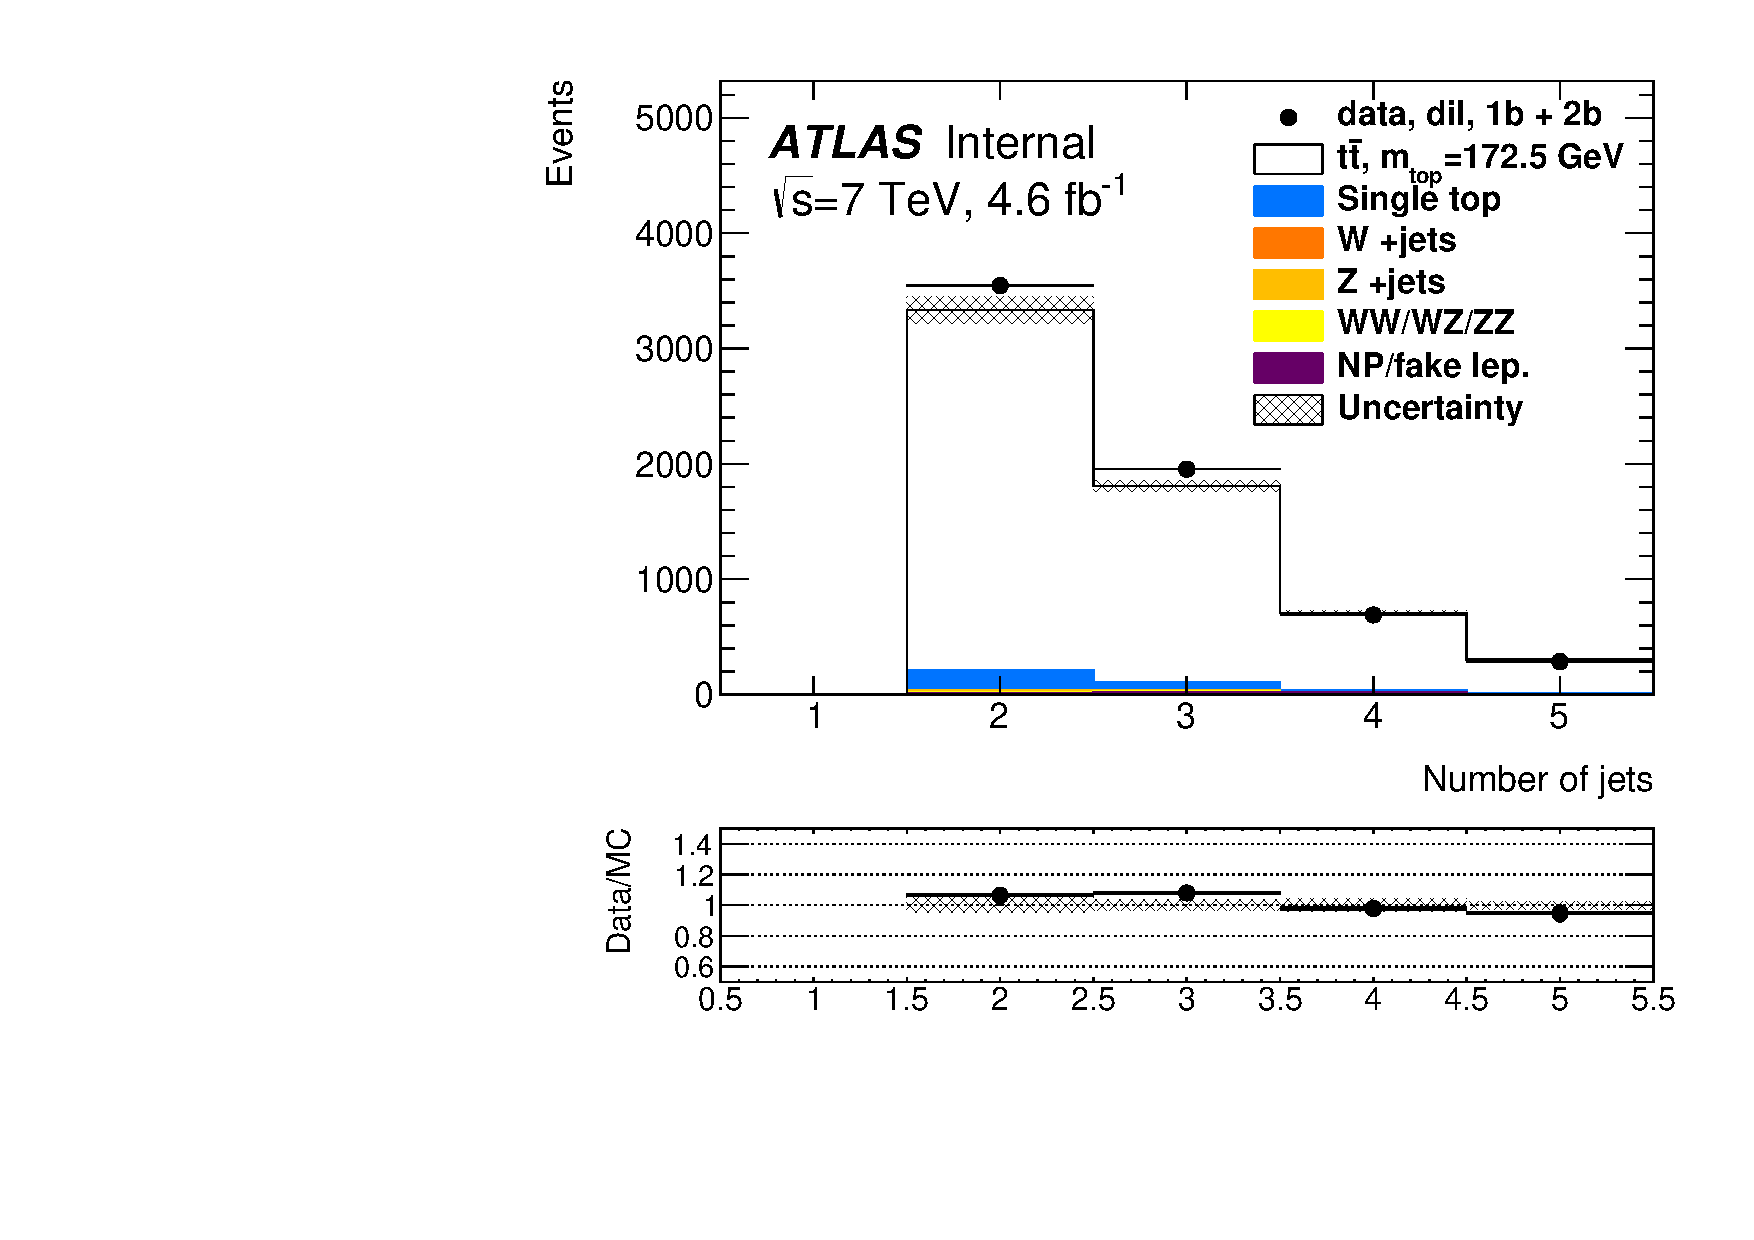
\includegraphics[width=0.49\textwidth]{./figs/Plot_3dTMT_dataMC_finalnjet_s1725_seltype5.pdf}
  \label{sfig:llnjets}
}
\subfloat[Number of \btagged\ jets]{
  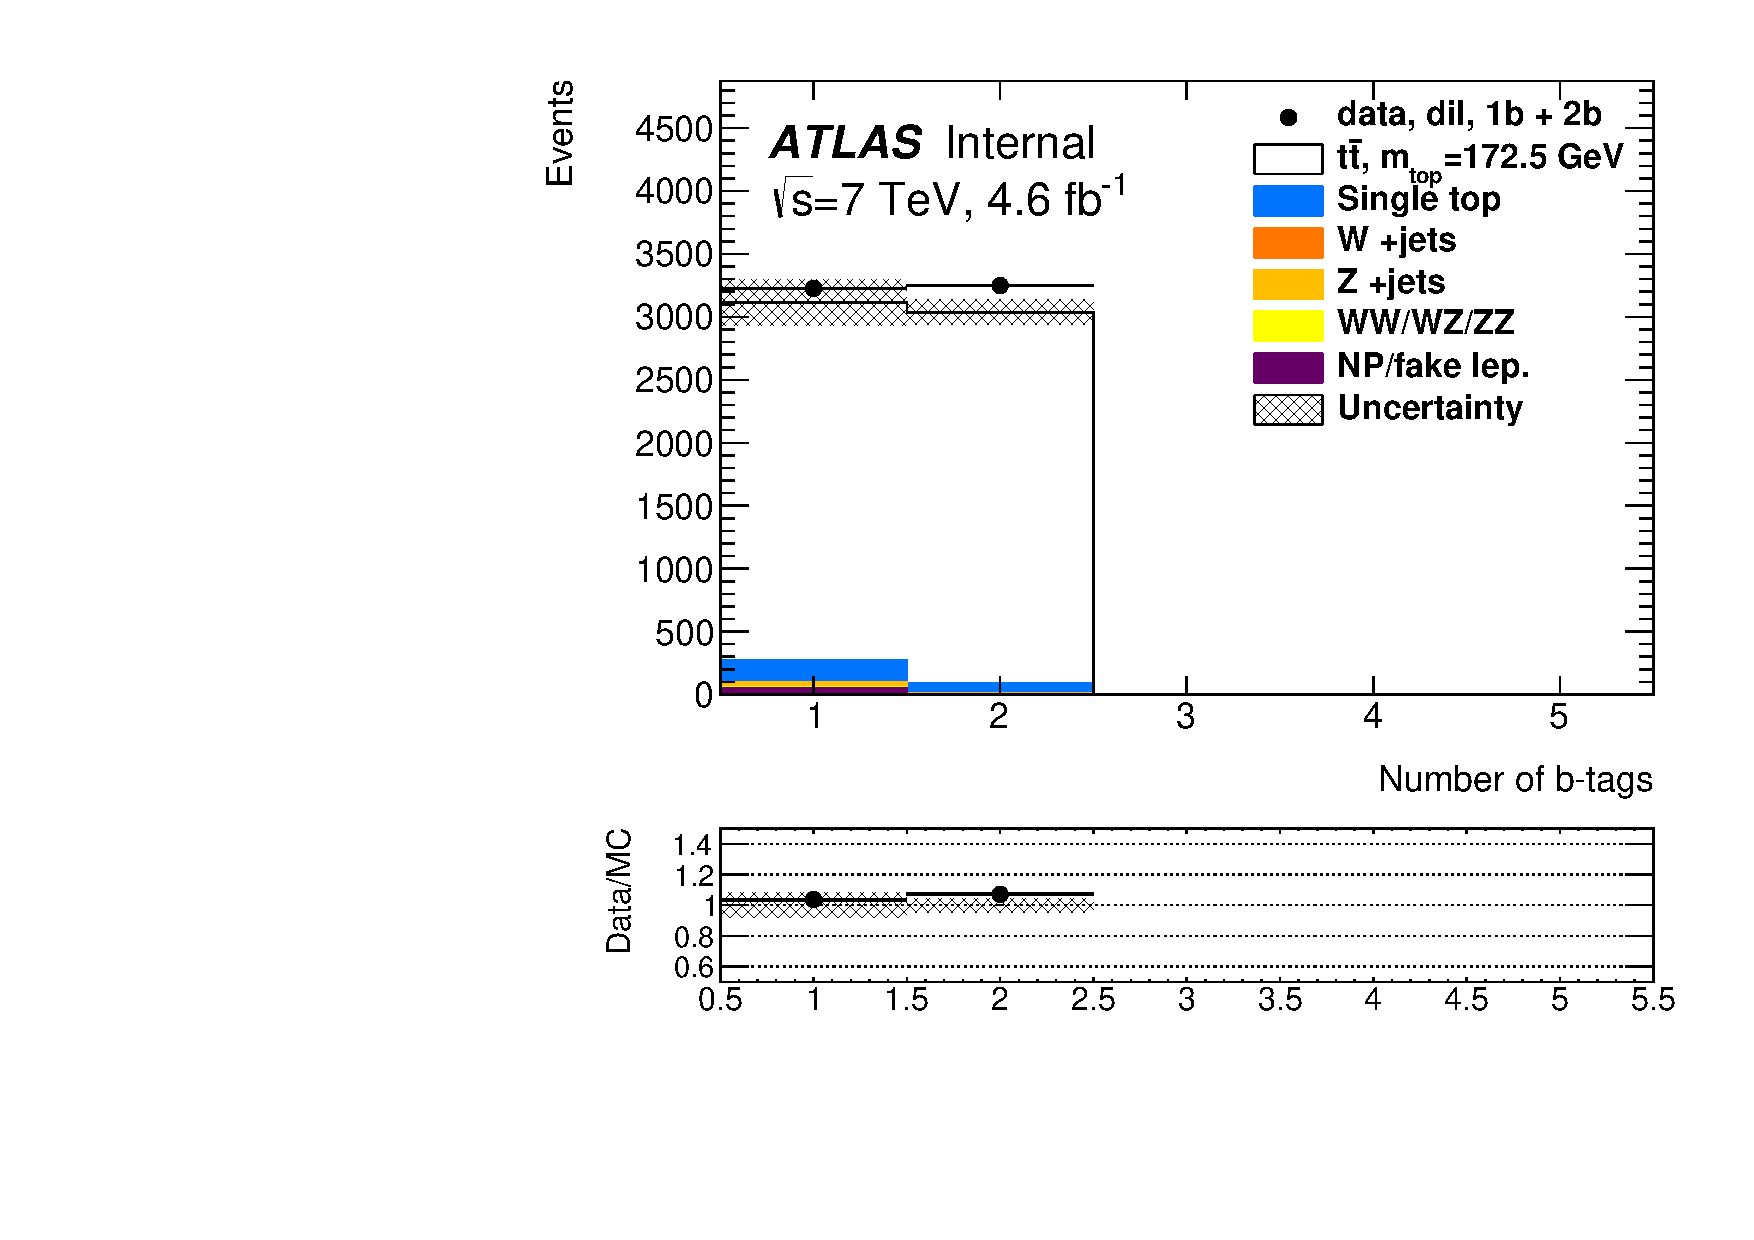
\includegraphics[width=0.49\textwidth]{./figs/Plot_3dTMT_dataMC_finalntag_s1725_seltype5.pdf}
  \label{sfig:llntaggedjets}
}
\hfill
\subfloat[\btagged\ jets \pt]{
  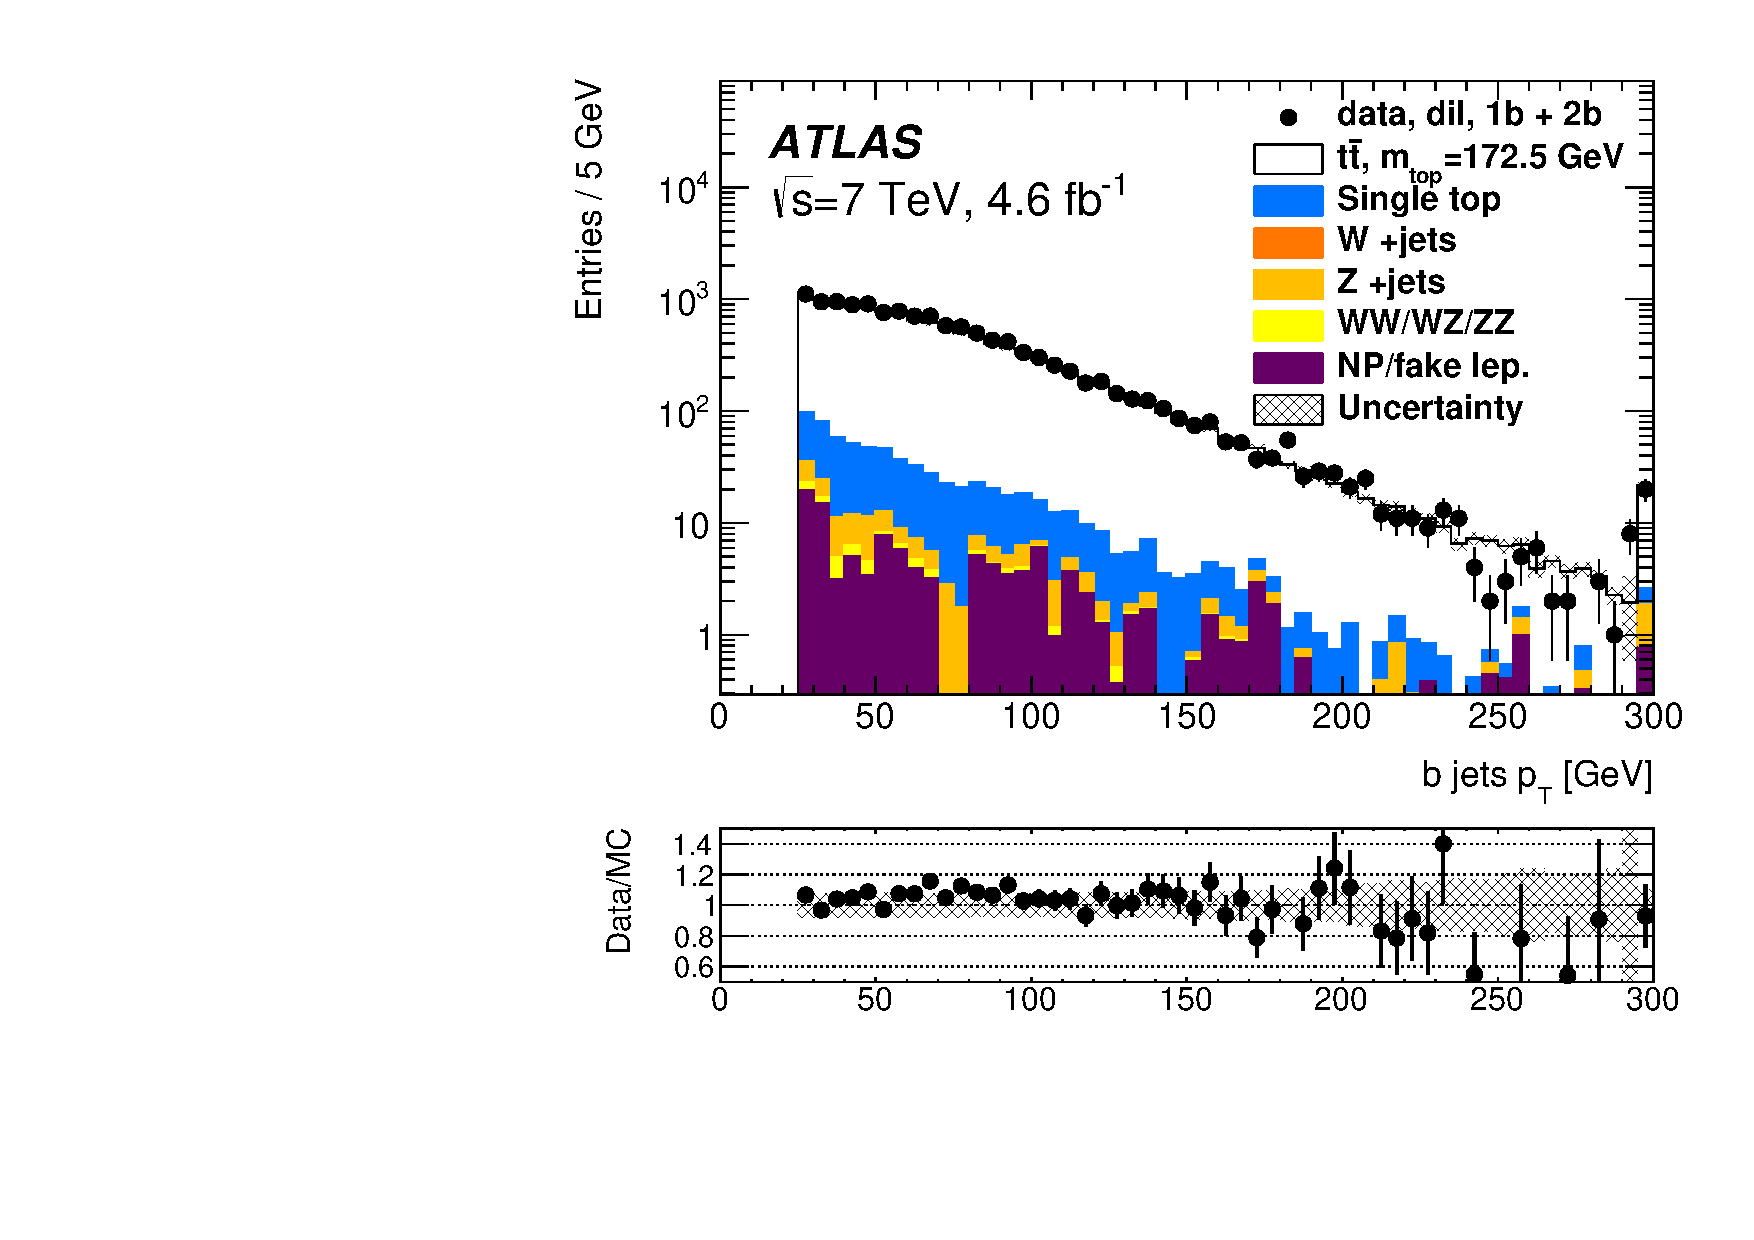
\includegraphics[width=0.49\textwidth]{./figs/Plot_3dTMT_dataMC_BjetPt_s1725_seltype5.pdf}
  \label{sfig:lltaggedjetspt}
}
\subfloat[Lepton \pt]{
  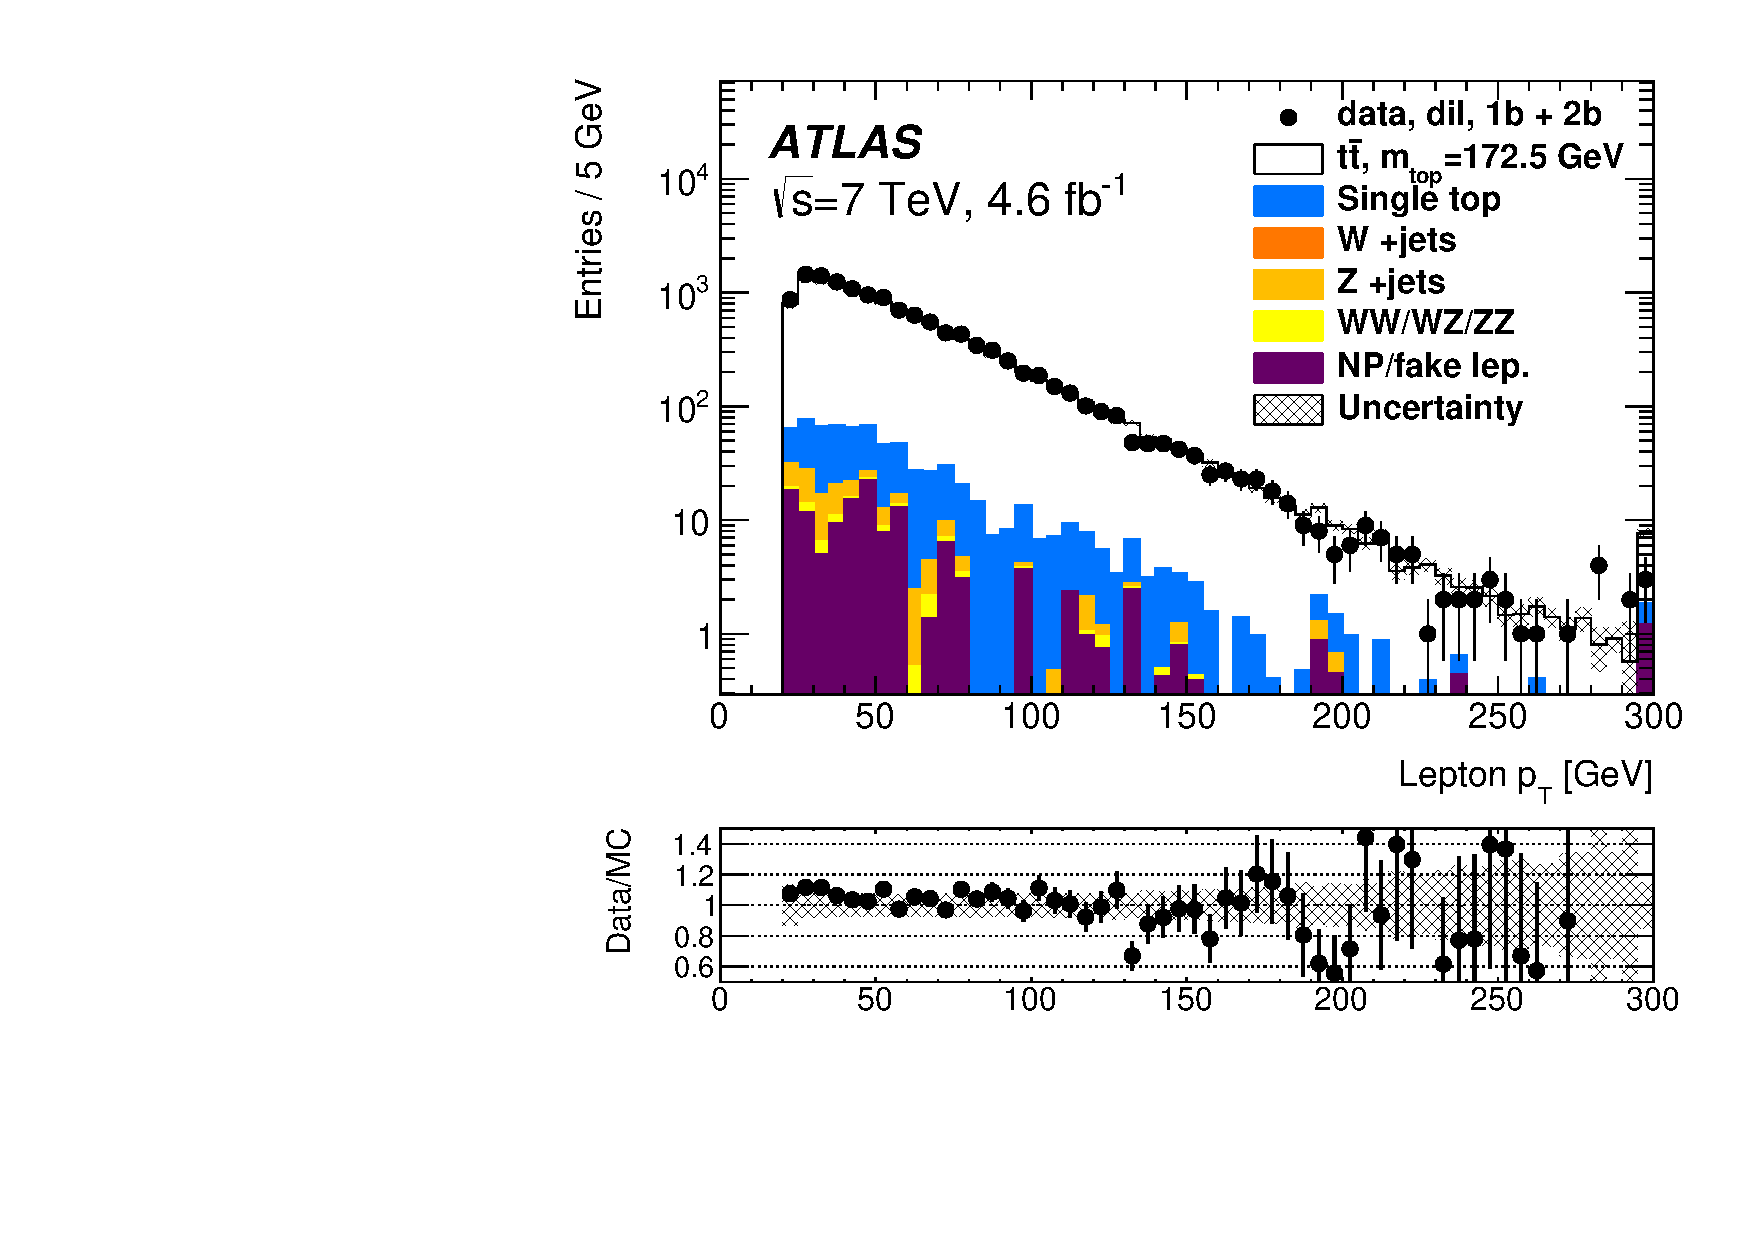
\includegraphics[width=0.49\textwidth]{./figs/Plot_3dTMT_dataMC_LepPt_s1725_seltype5.pdf}
  \label{sfig:llleptonspt}
}
\hfill
\subfloat[\btagged\ jets  $\eta$]{
  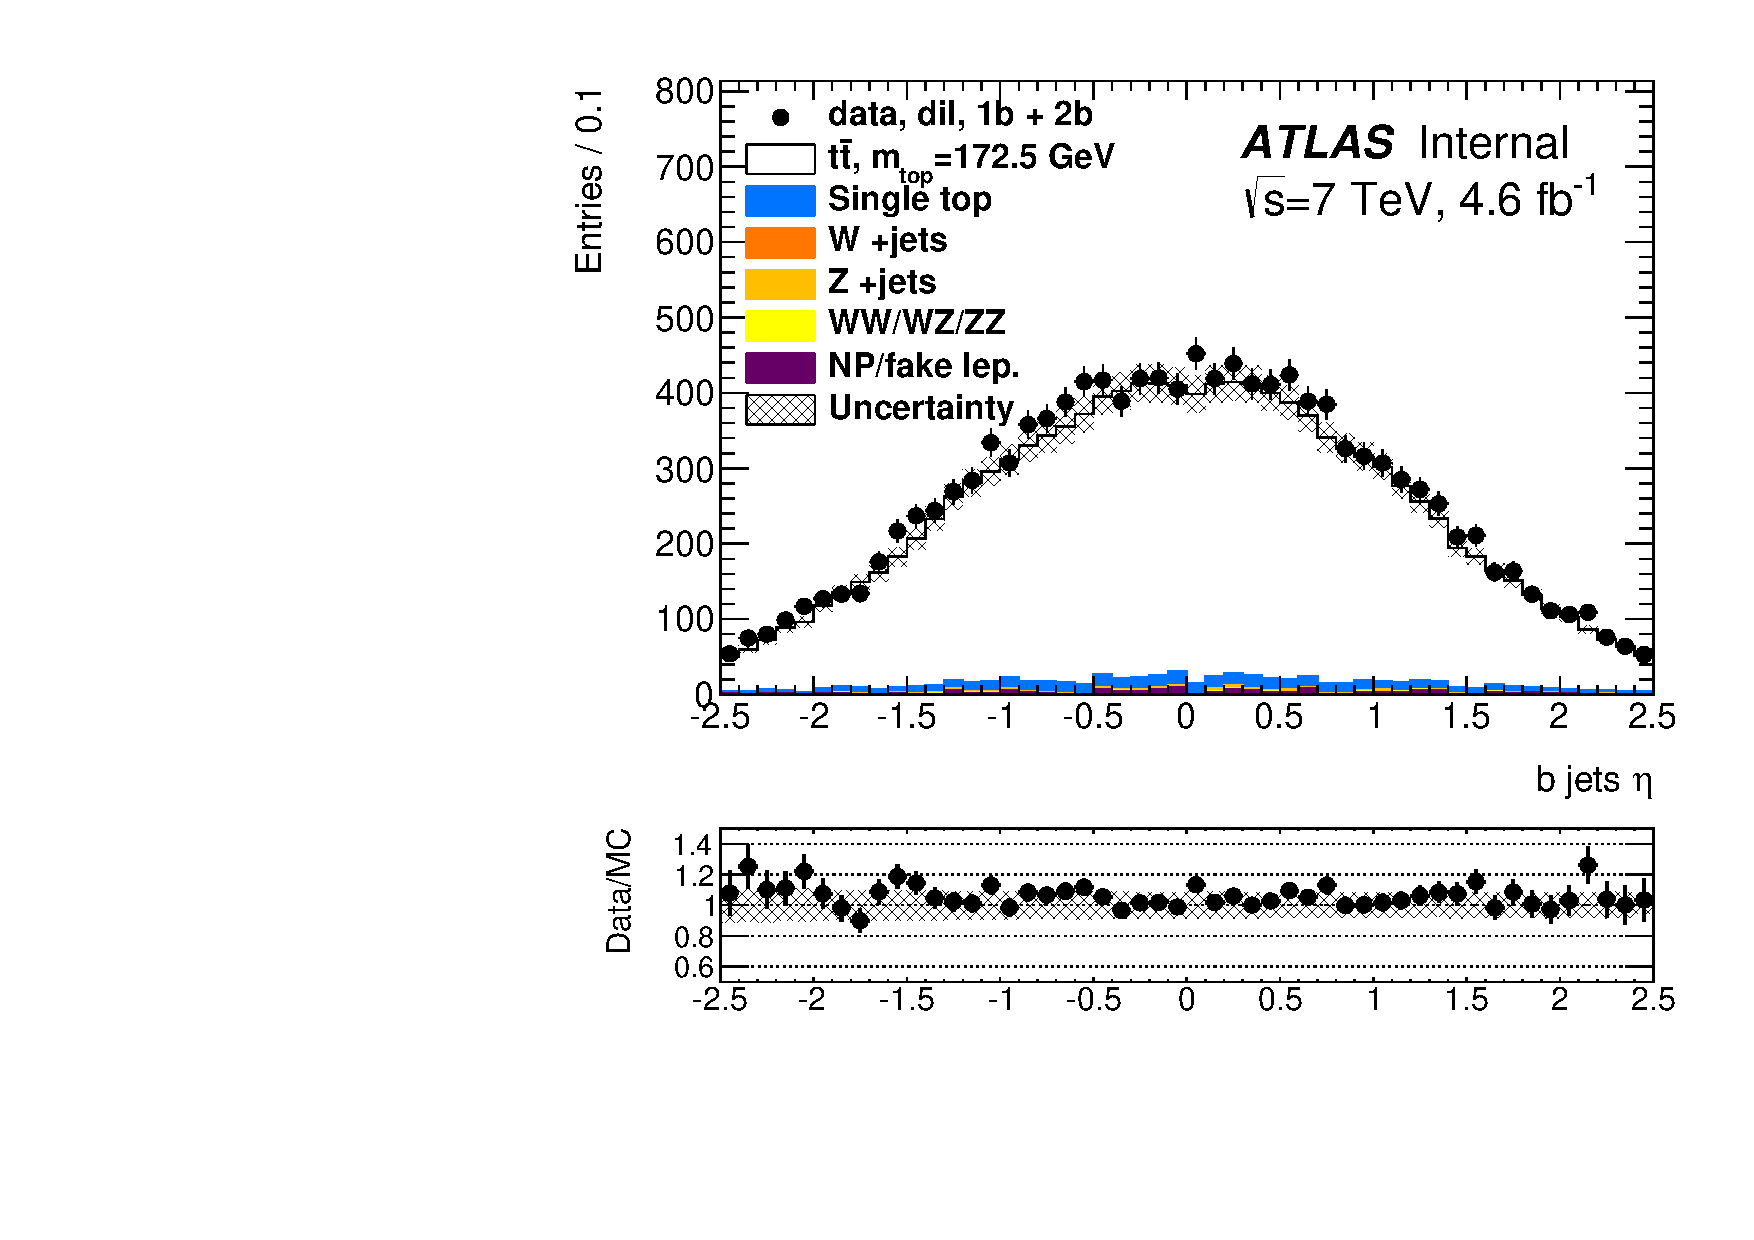
\includegraphics[width=0.49\textwidth]{./figs/Plot_3dTMT_dataMC_BjetEta_s1725_seltype5.pdf}
  \label{sfig:lltaggedjetseta}
}
\subfloat[Lepton $\eta$]{
  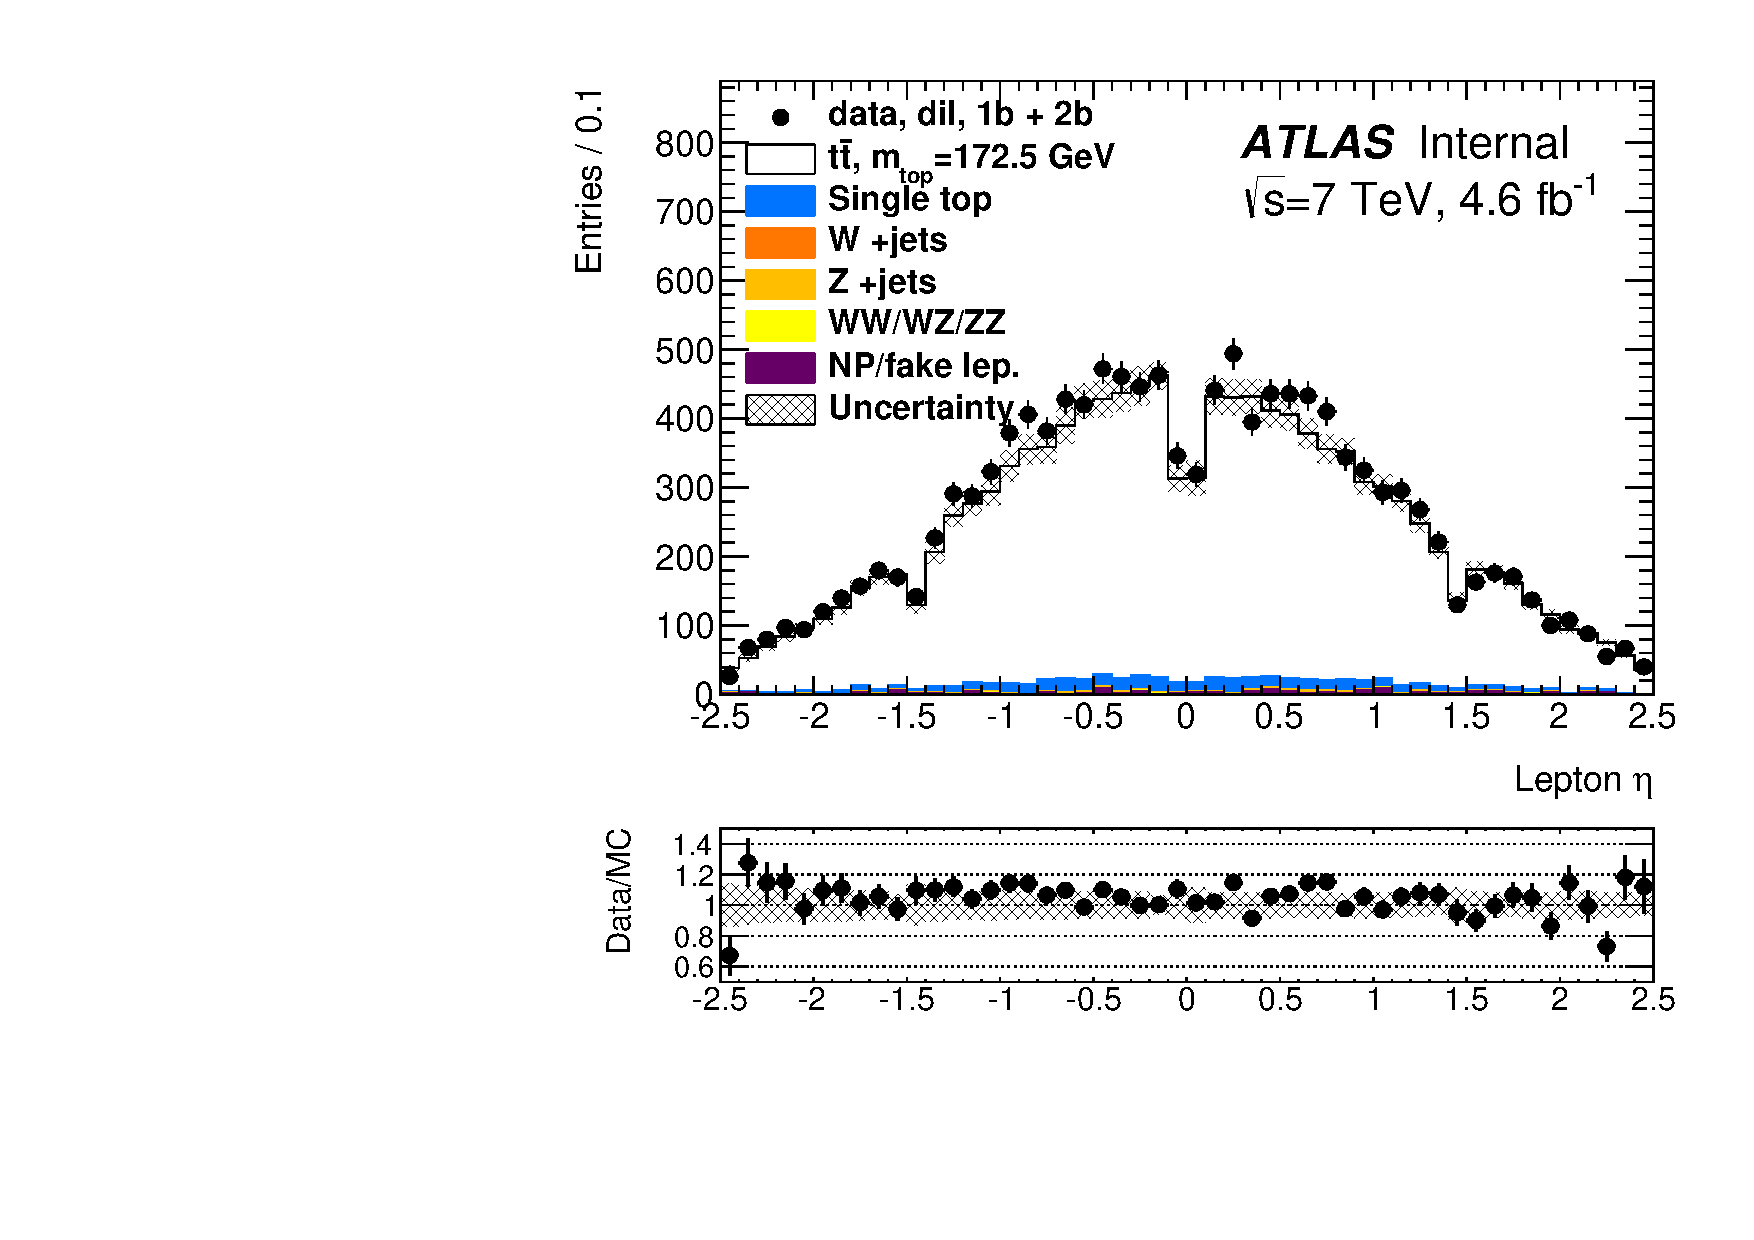
\includegraphics[width=0.49\textwidth]{./figs/Plot_3dTMT_dataMC_LepEta_s1725_seltype5.pdf}
  \label{sfig:lltaggedleptonseta}
}
\hfill
\caption[Data to \gls{MC} comparison for $\sqrts=7$~\TeV\ data: direct observables]{
\Fig{s}~\subref{sfig:llnjets} and \subref{sfig:llntaggedjets} show the jet and \btagged\ jet multiplicity, \fig{s}~(c, d) and (e, f) show the distributions of the lepton and \btagged\ jets \pt\ and $\eta$. 
%
The data are shown by the points with statistical uncertainty bars, and the predictions are shown by the solid histograms. 
%
The hatched area is the combined uncertainty on the prediction described in \sect~\ref{sect:evtyields7TeV}, and the rightmost bin contains the overflow, if present. 
%
For each figure, the ratio of the data to the \gls{MC} prediction is also presented.
%
  \label{fig:DLdataMCcomp7TeV}}
\end{figure*}
%%%%%%%%%%%%%%%%%%%%%%%%%%%%%%%%%%%%%%%%%%%%%%%%%%%%%%%%%%%%%%%%%%%%%%%%%%%%%%%
%
%%%%%%%%%%%%%%%%%%%%%%%%%%%%%%%%%%%%%%%%%%%%%%%%%%%%%%%%%%%%%%%%%%%%%%%%%%%%%%%
\begin{figure*}[tbp!]
\centering
\subfloat[\met]{
  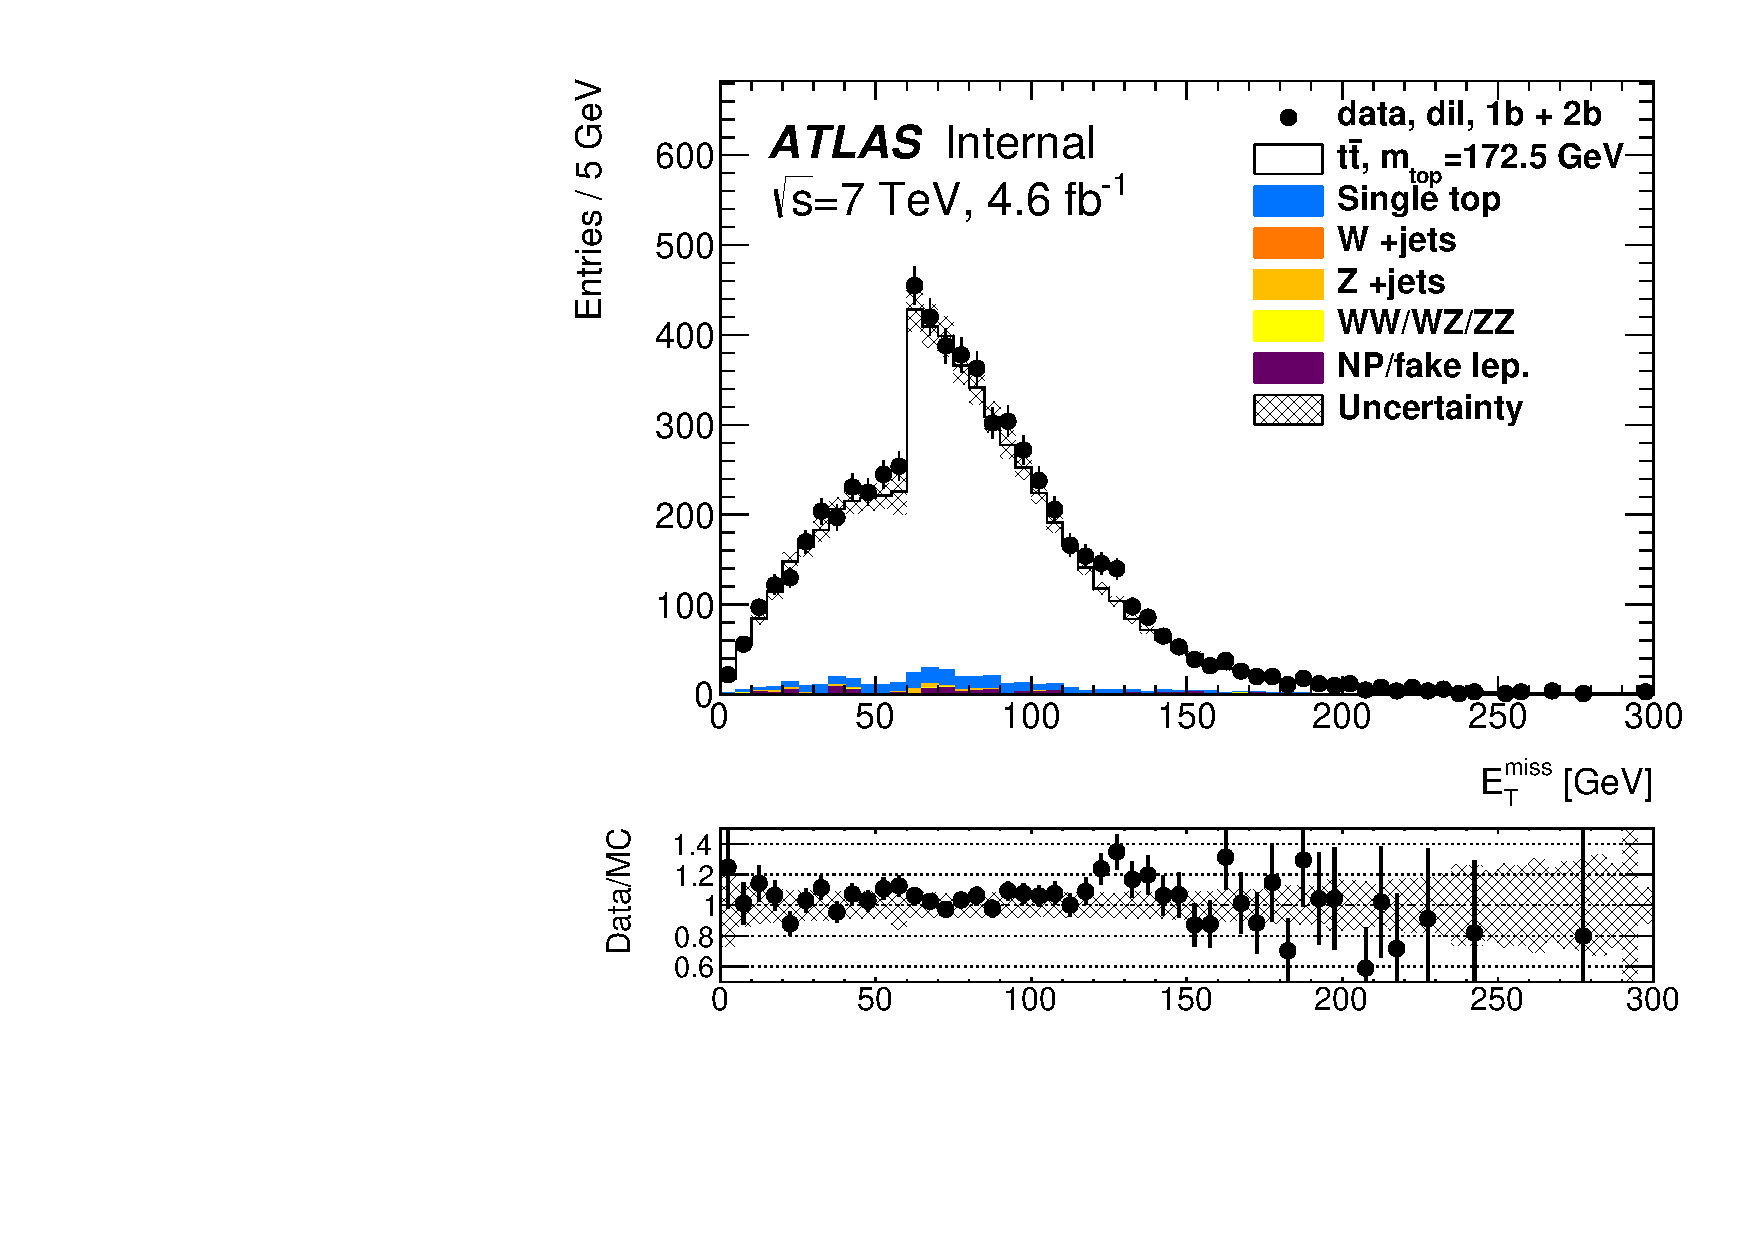
\includegraphics[width=0.49\textwidth]{./figs/Plot_3dTMT_dataMC_Met_s1725_seltype5.pdf}
  \label{sfig:llmet}
}
\subfloat[\mlbr]{
  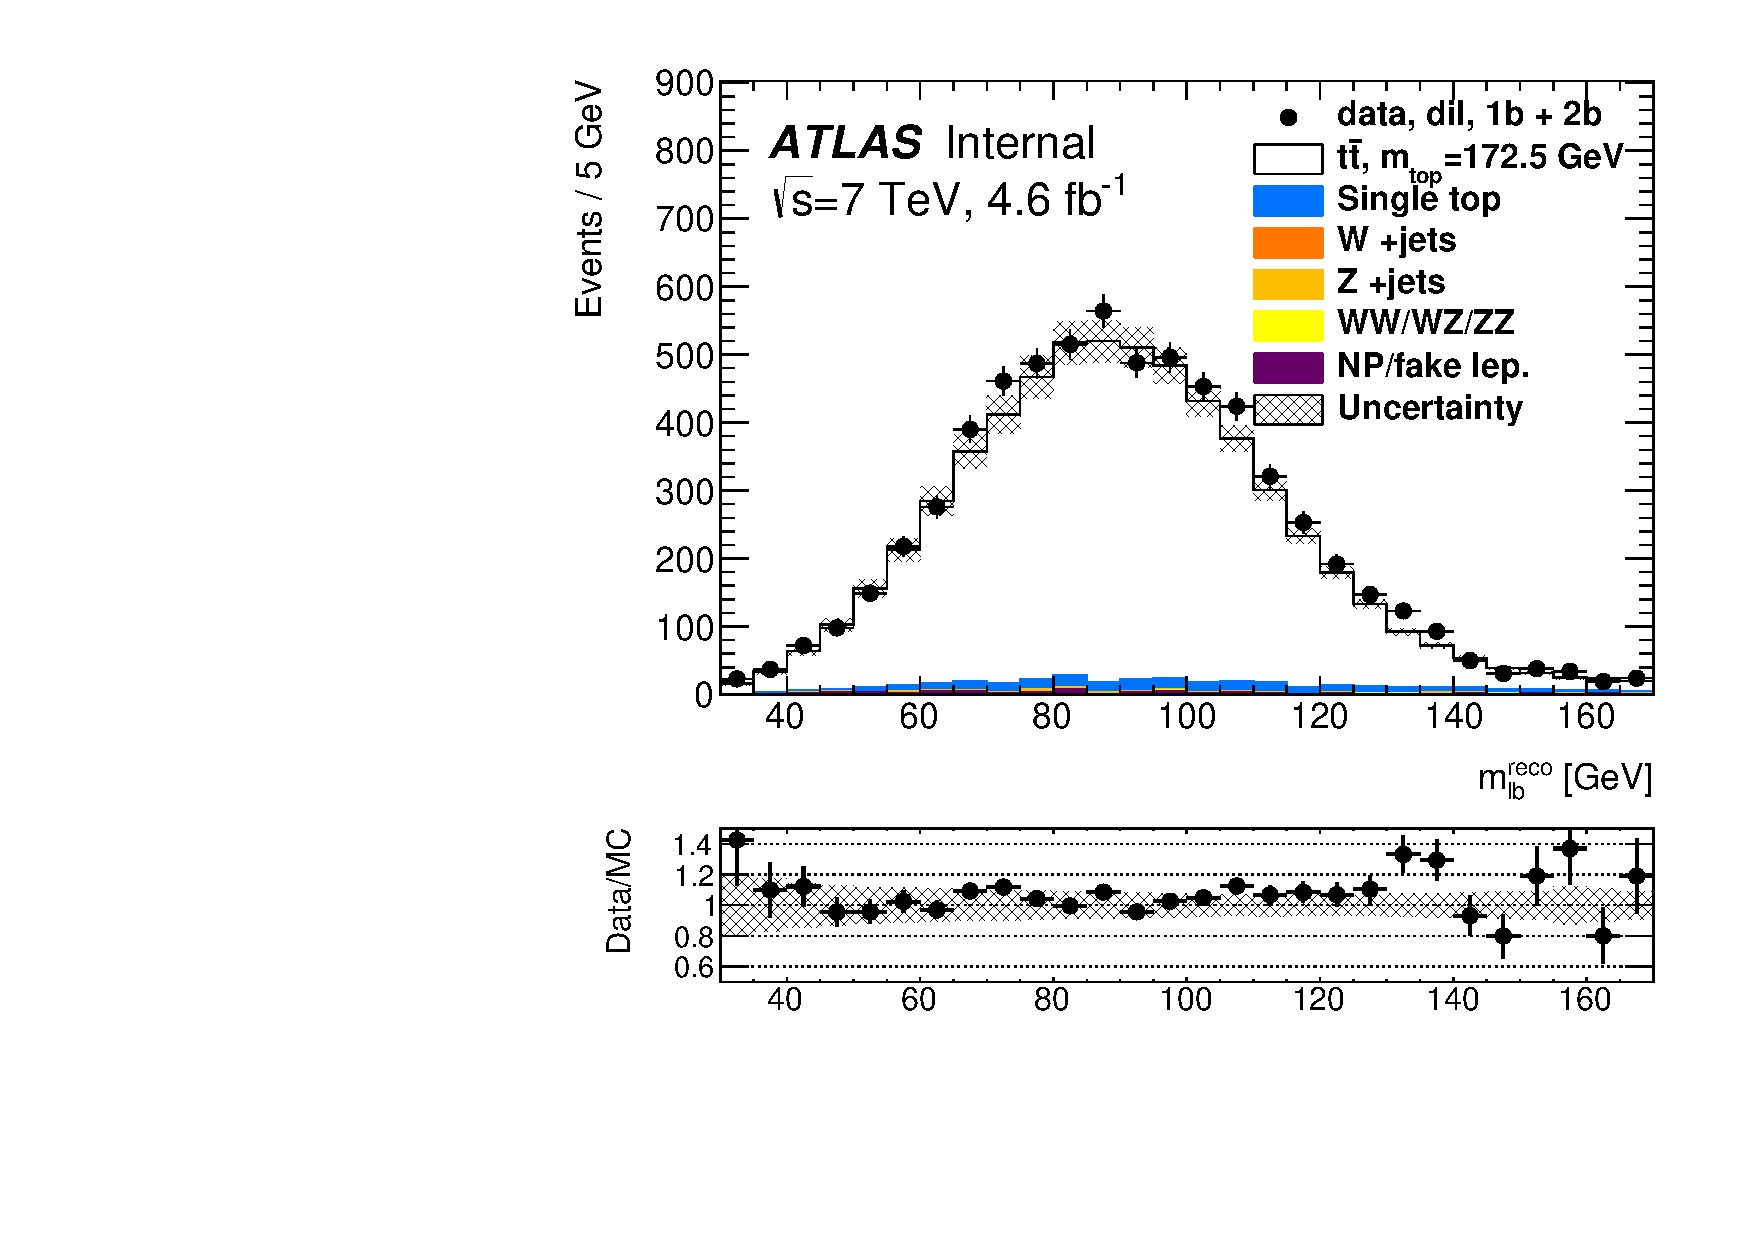
\includegraphics[width=0.49\textwidth]{./figs/Plot_3dTMT_dataMC_mlb_s1725_seltype5.pdf}
  \label{sfig:llmlb}
}
\hfill
\subfloat[\ptbb]{
  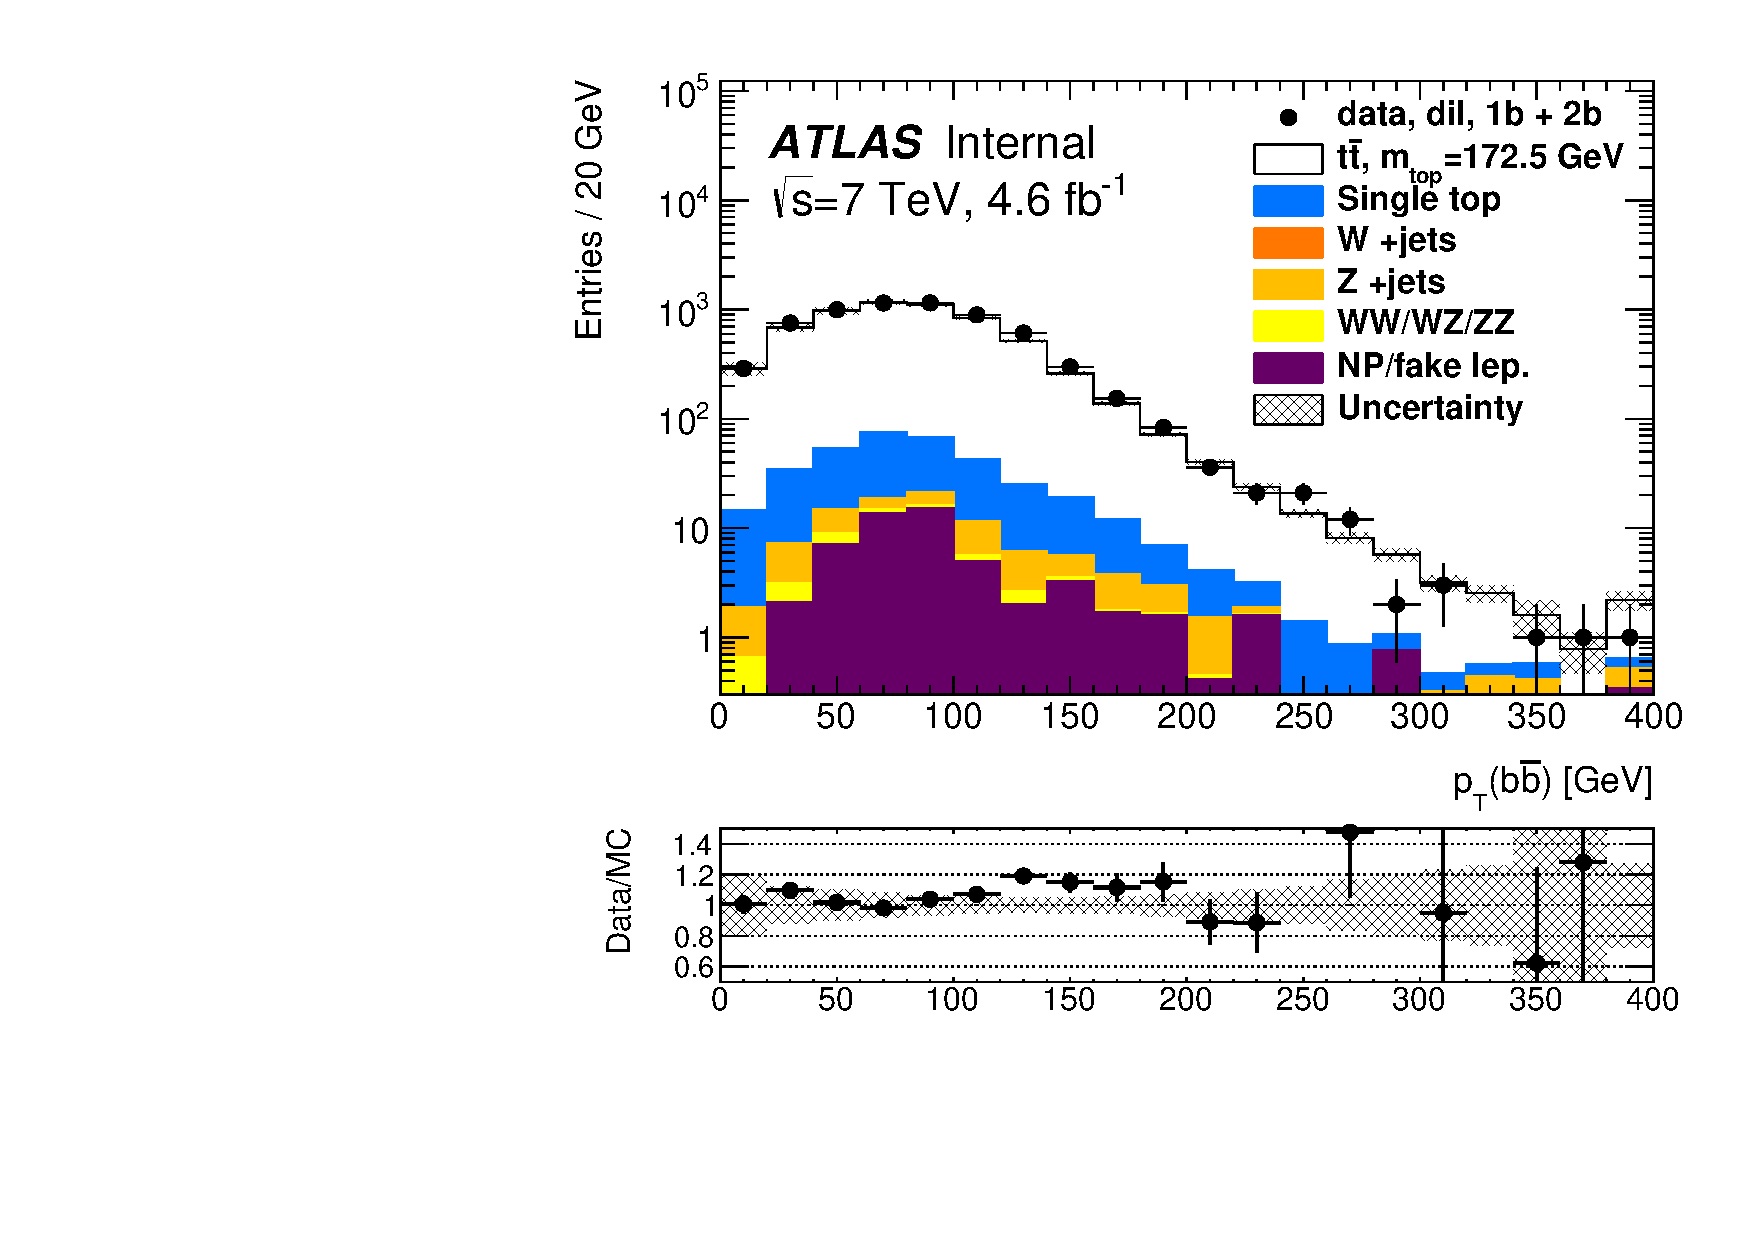
\includegraphics[width=0.49\textwidth]{./figs/Plot_3dTMT_dataMC_pTbb_s1725_seltype5.pdf}
  \label{sfig:llptbb}
}
\subfloat[\ptll]{
  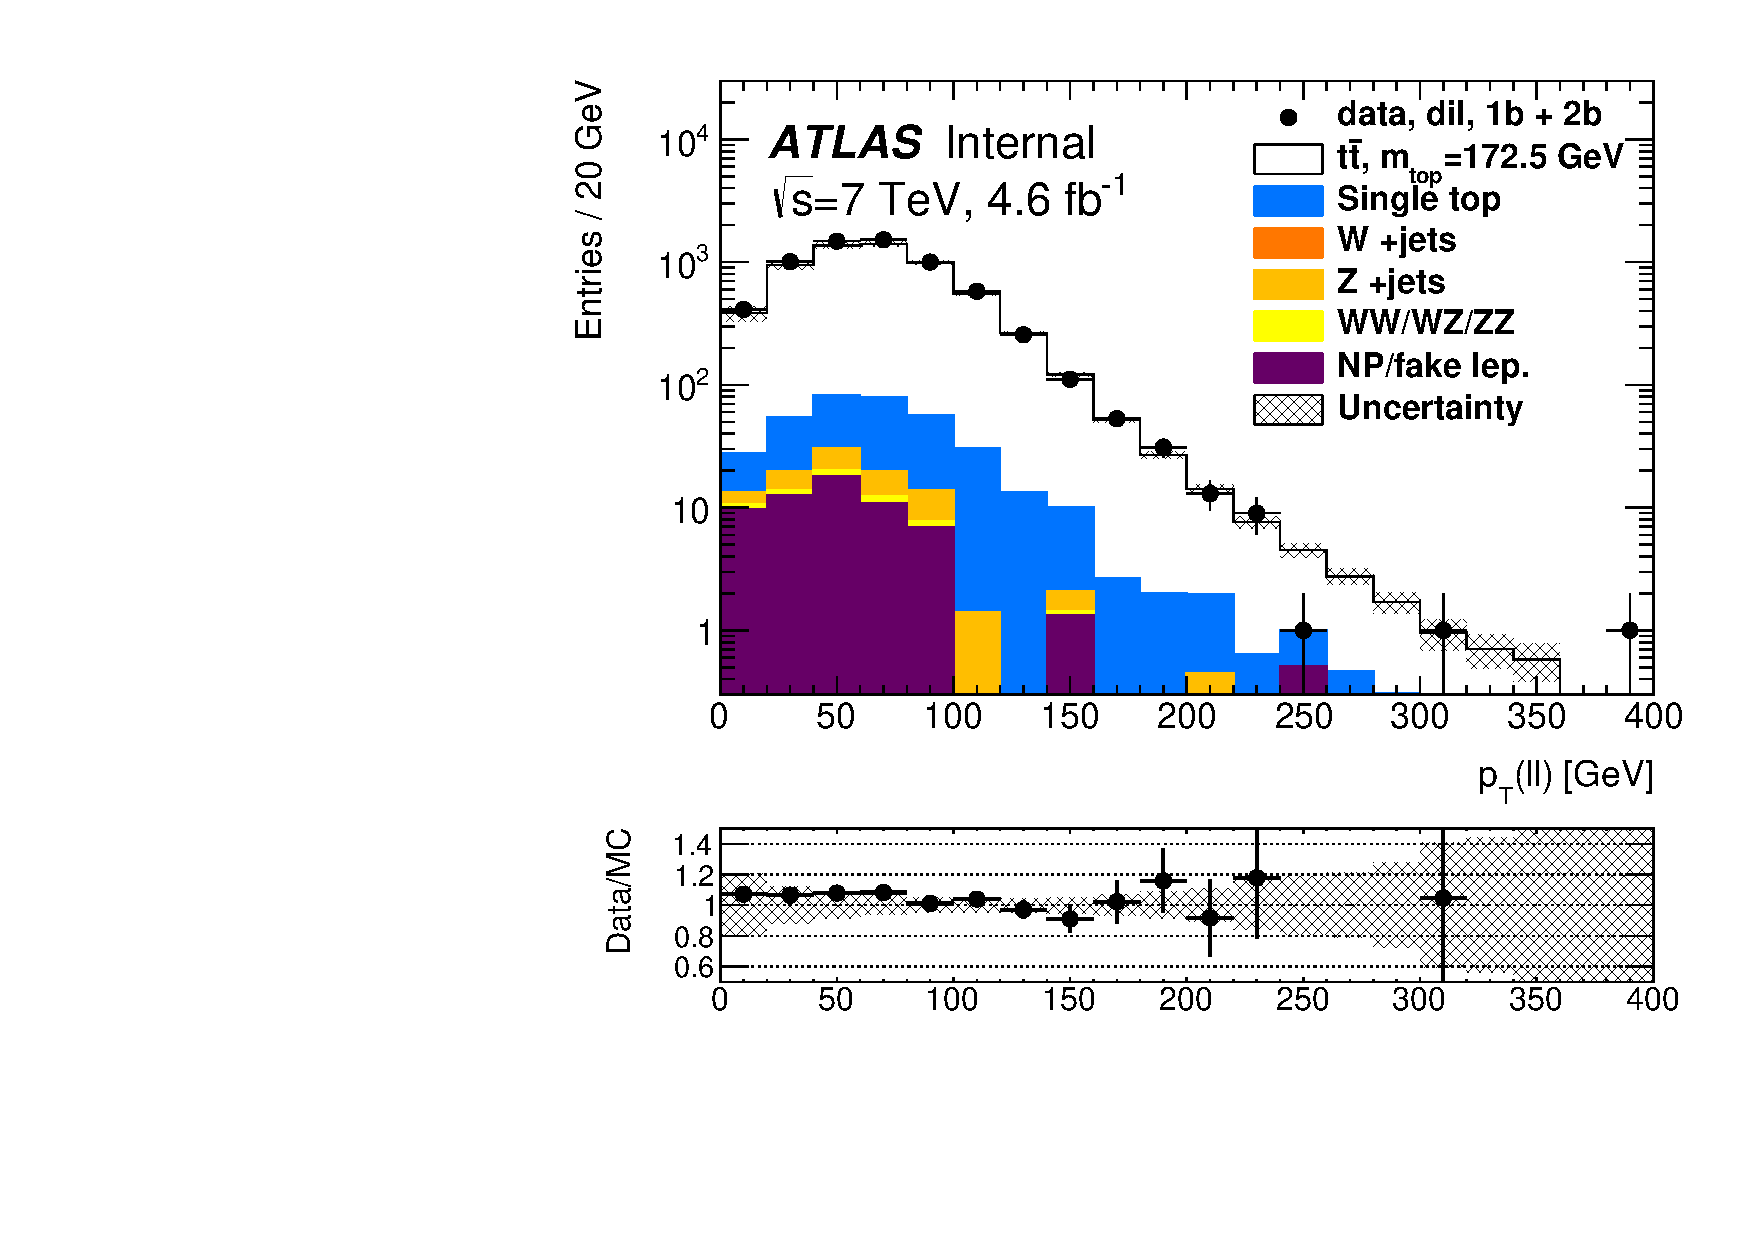
\includegraphics[width=0.49\textwidth]{./figs/Plot_3dTMT_dataMC_pTll_s1725_seltype5.pdf}
  \label{sfig:llptll}
}
\hfill
\caption[Data to \gls{MC} comparison for $\sqrts=7$~\TeV\ data: derived observables]{
%
Same as \fig~\ref{fig:DLdataMCcomp7TeV} but \fig{s}~\subref{sfig:llmet} and \subref{sfig:llmlb} show the \met\ and \mlbr\ distributions. \Fig{s}~\subref{sfig:llptbb} and \subref{sfig:llptll} show the \pt\ distributions of the dijet and \dil\ systems.
%
  \label{fig:DLdataMCcomp7TeV2}}
\end{figure*}
%%%%%%%%%%%%%%%%%%%%%%%%%%%%%%%%%%%%%%%%%%%%%%%%%%%%%%%%%%%%%%%%%%%%%%%%%%%%%%%


































\clearpage






\section{The template method}
The analysis method employed in this work is the template method. 
%
Templates are simulated distributions of an estimator, constructed for a number of discrete values of the parameter under study, in this case for different \mt values. 
%
Appropriate functions are then fitted to these templates, interpolating between different input values of the physics parameter. 
%
The remaining parameters of the functions are fixed by a simultaneous fit to all templates, imposing linear dependences of the parameters on \mt. 
%
The resulting template fit function has \mt as the only free parameter and an unbinned likelihood maximisation yields the value of \mt\ that best describes the data. 
%
This procedure is detailed in the following.












\subsection{Construction of the likelihood function}
\label{sect:like7TeV}

The signal templates are distributions of \mlbr, based on independent \gls{MC} samples, using different input values of \mt in the range of $167.5$ to $177.5$~\GeV\ in steps of $2.5$~\GeV.
%
The \mlbr\ estimator distribution and its dependency on the underlying \gls{MC} \mt\ value are shown in \fig~\ref{fig:templtop7TeV} for events with exactly two \btagged\ jets. 
%
%%%%%%%%%%%%%%%%%%%%%%%%%%%%%%%%%%%%%%%%%%%%%%%%%%%%%%%%%%%%%%%%%%%%%%%%%%%%%%%
\begin{figure*}[tbp!]
\centering
% \subfloat[\mlbr\ for exactly two \btagged\ jets]{
	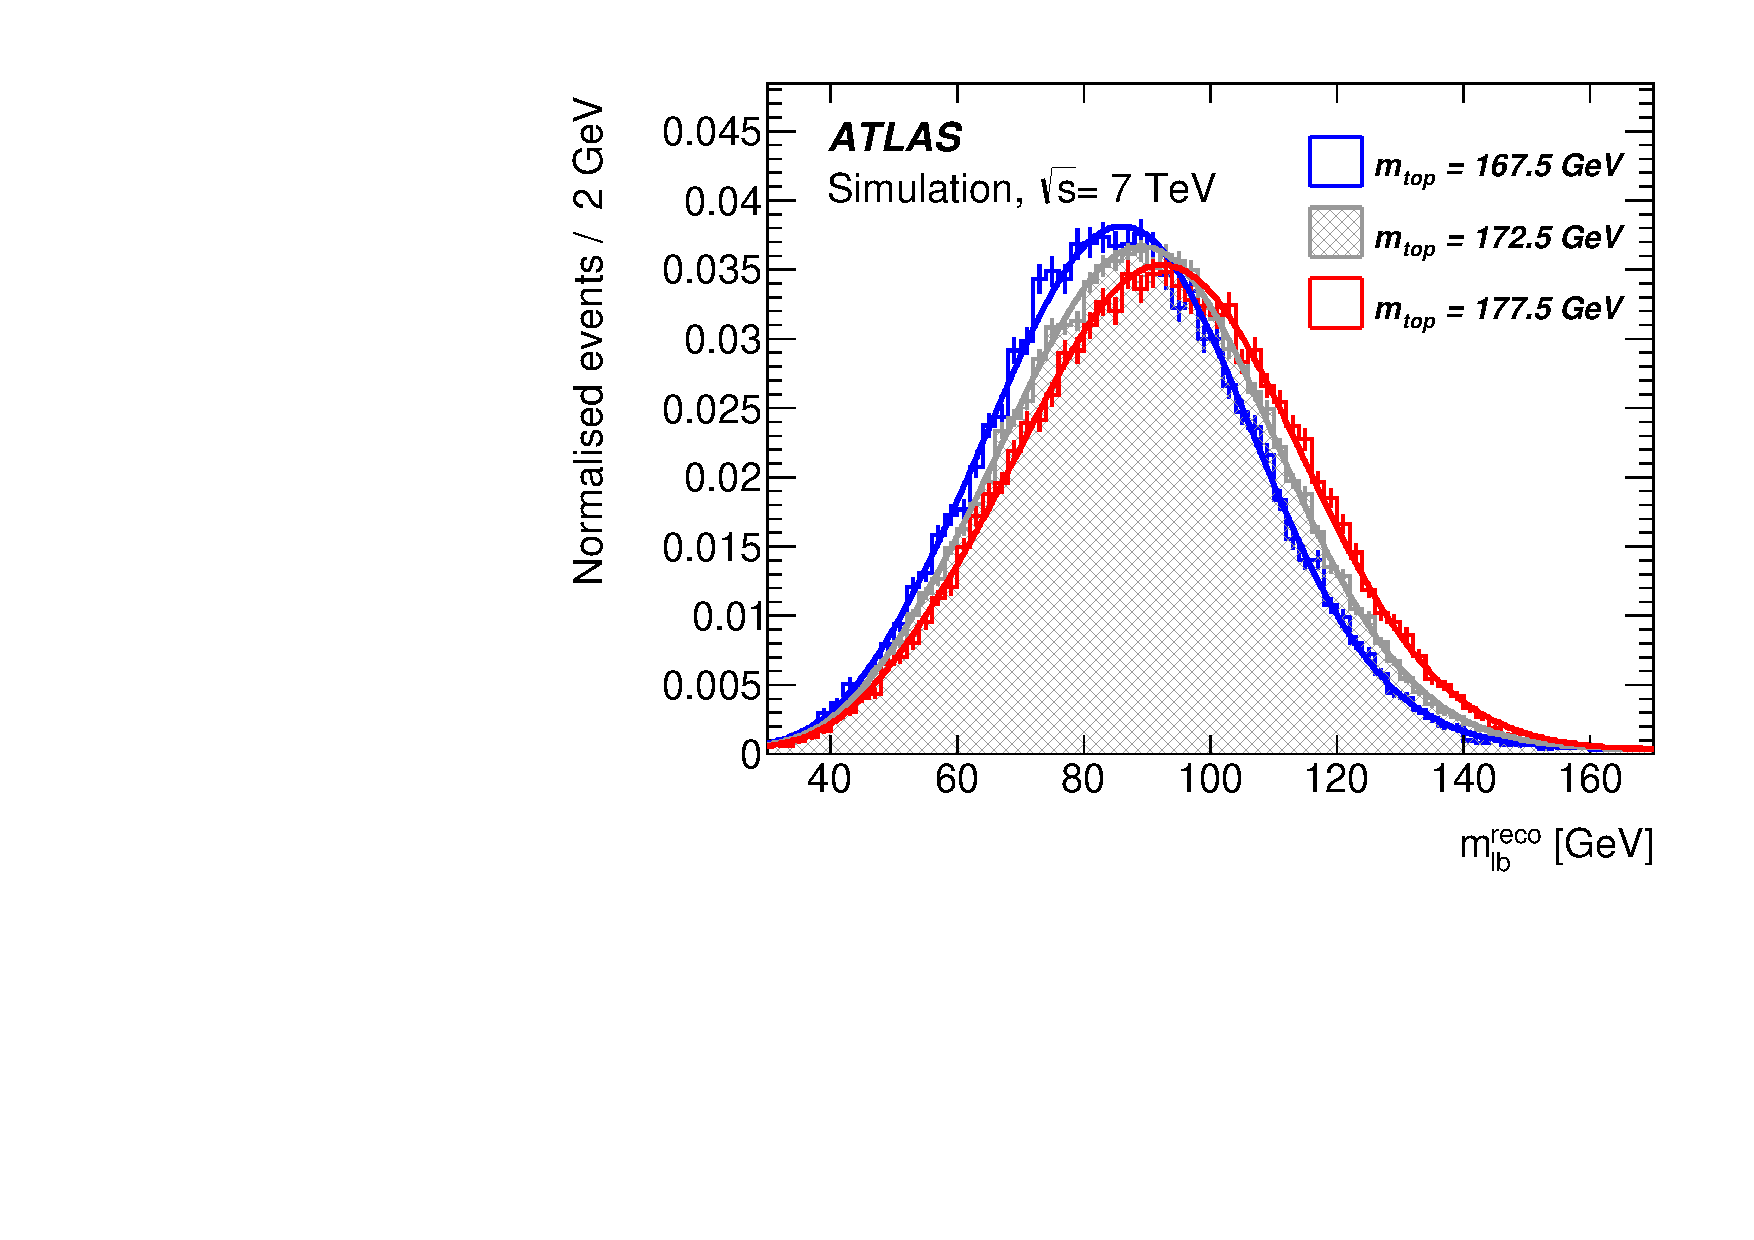
\includegraphics[width=0.6\textwidth]{./figs/MC_fit_wp75_mlb_overlaid_ele0_dep0.pdf}
	% \label{sfig:mlbrmtop}
% }
\caption[Template fit functions for $\sqrts=7$~\TeV\ data]{
%
The distribution of \mlbr\ for different values of the input \mt\ for \gls{MC} signal events with exactly two \btagged\ jets. 
%
The corresponding \glspl{pdf} are displayed on top of the distributions.
%
\label{fig:templtop7TeV}}
\end{figure*}
%%%%%%%%%%%%%%%%%%%%%%%%%%%%%%%%%%%%%%%%%%%%%%%%%%%%%%%%%%%%%%%%%%%%%%%%%%%%%
%
%
The sum of a Gaussian and a Landau function is fitted to the \mlbr\ signal templates produced with different \mt\ values. 
%
A Landau function is fitted to the background template. 
%
Since the single \tquark\ contribution with its \tquark\ mass dependence is included in the signal, the background templates are insensitive to and not parametrised as a function of \mt. 
%
The fits are done separately for events with exactly one or exactly two \btagged\ jets. 
%
After verifying that all fit parameters of the separate fits depend linearly on \mt, the linearity is imposed and used to fix all other parameters in a combined fit to all templates. An example for this procedure can be found in \reference~\cite{Maier2012}.
%
The resulting signal and background \glspl{pdf} are used in an unbinned likelihood fit to the data.
%
The likelihood function, maximised for $N$ data events, is
%
%%%%%%%%%%%%%%%%%%%%%%%%%%%%%%%%%%%%%%%%%%%%%%%%%%%%%%%%%%%%%%%%%%%%%%%%%%%%%%%
\[
\Like(\mt, \fbkg) = 
\prod_{i=1}^{N} 
\left[ (1-\fbkg)\cdot \Ptopsig(\mlbri \,\vert\, \mt) + \fbkg \cdot \Ptopbkg(\mlbri) \right],
\]
%%%%%%%%%%%%%%%%%%%%%%%%%%%%%%%%%%%%%%%%%%%%%%%%%%%%%%%%%%%%%%%%%%%%%%%%%%%%%%%
%
with \Ptopsig\ and \Ptopbkg\ denoting the signal and background \glspl{pdf} and \fbkg\ the fraction of background events in the selected data sample.

% %
%%%%%%%%%%%%%%%%%%%%%%%%%%%%%%%%%%%%%%%%%%%%%%%%%%%%%%%%%%%%%%%%%%%%%%%%%%%%%%%%%%%%%%
\begin{figure*}[tbp!]
\centering
\subfloat[\mt\ residual]{
  % \includegraphics[width=0.49\textwidth,trim={460 210 0 0},clip]{./figs/Plot_Pexp_RlbCalo_dim0_shape_2_ele2_bkgfr_002wc_501_pe_4600_invpb_summary.pdf}
  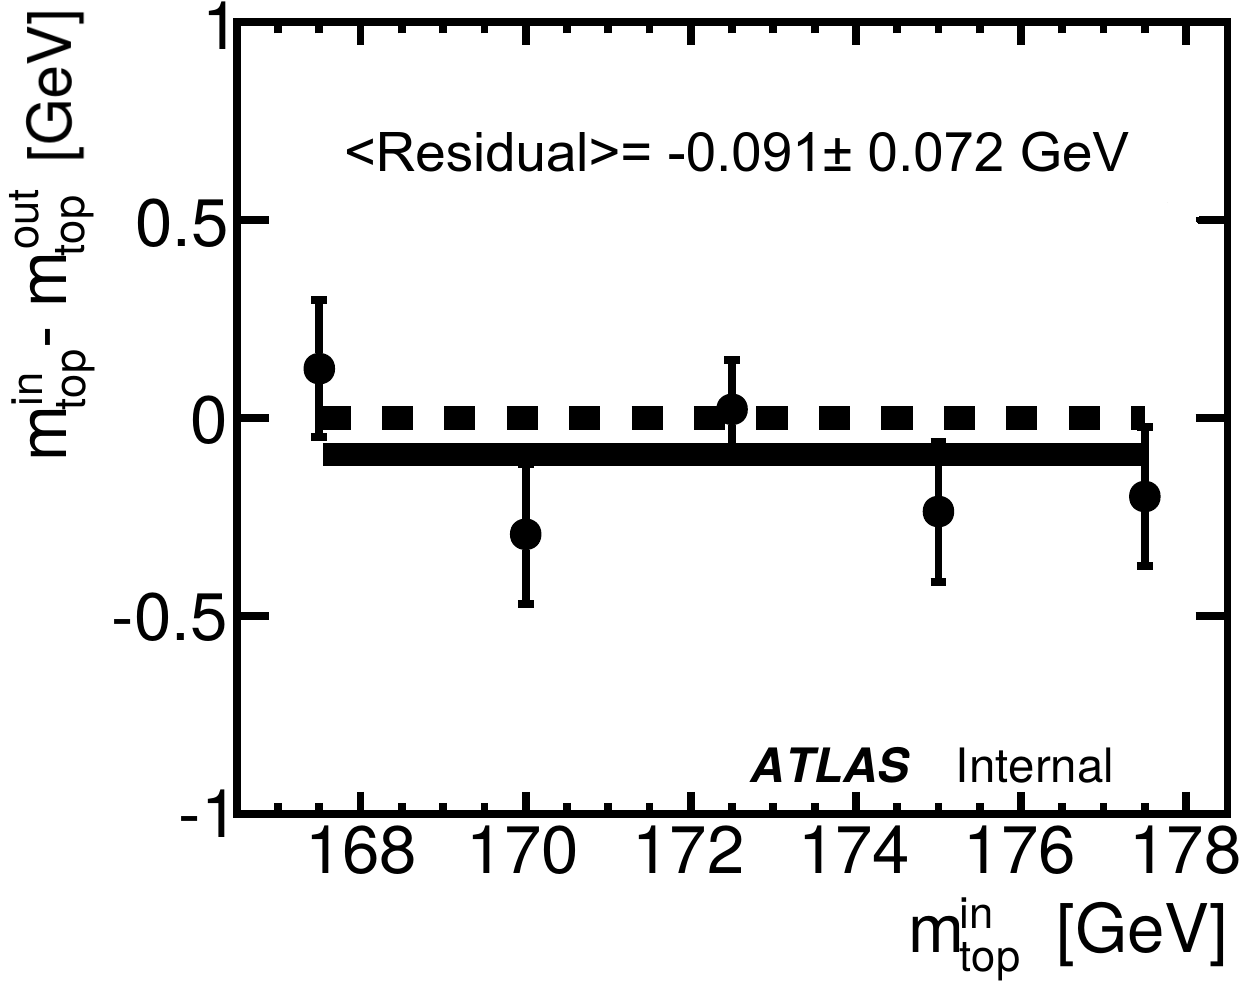
\includegraphics[height=0.4\textwidth]{./figs/bias7TeV.png}
  \label{sfig:bias7TeV}
}
\subfloat[Pull width]{
  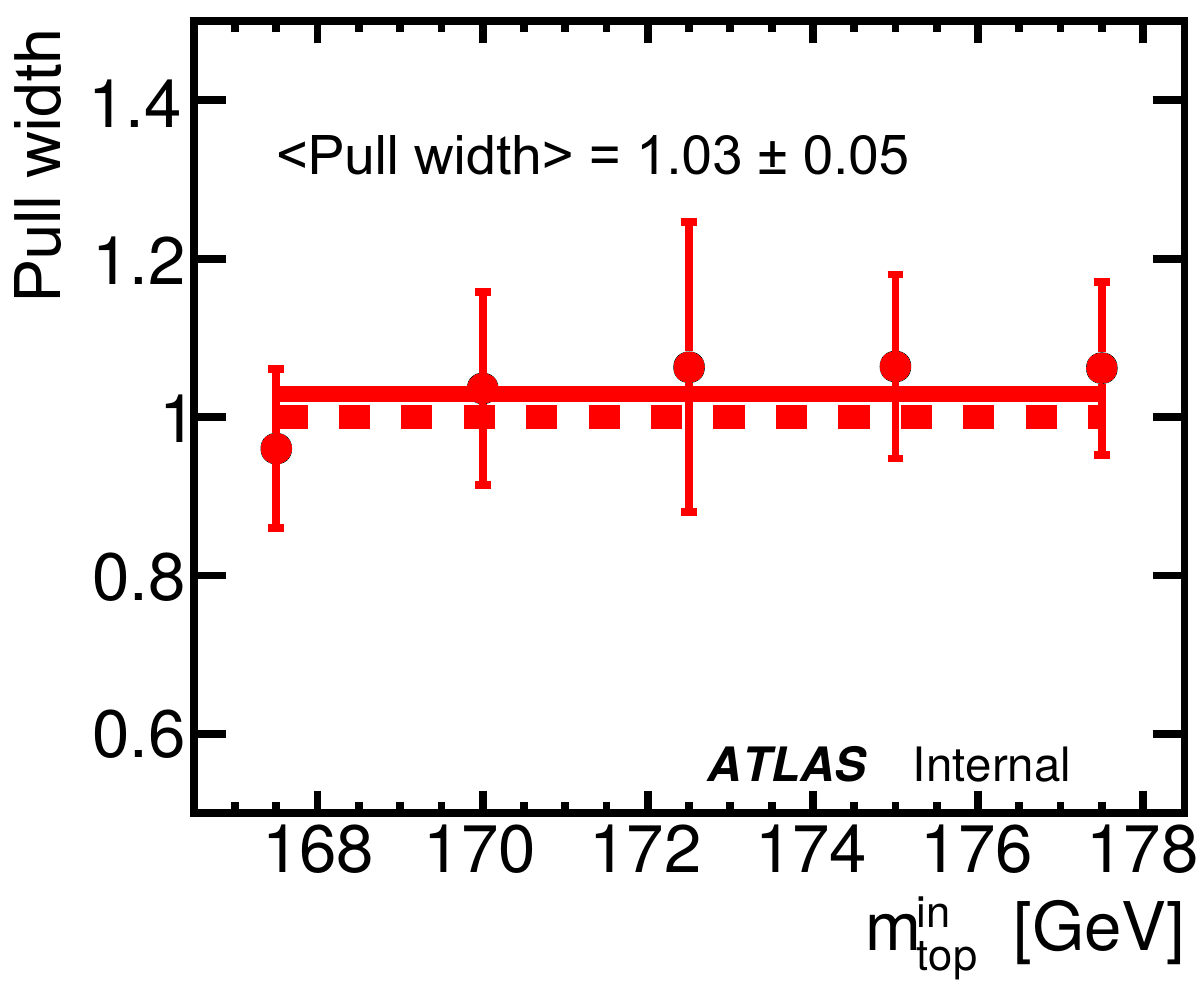
\includegraphics[height=0.4\textwidth]{./figs/pullwidth7TeV.png}
  \label{sfig:pullwidth7TeV}
}
\caption[\mt\ residuals and pull widths for $\sqrts=7$~\TeV\ data]{
%
\Fig~\subref{sfig:bias7TeV} shows the \mt\ residuals observed when applying the method to the respective input templates and \fig~\subref{sfig:pullwidth7TeV} shows the pull distribution width.
%
The dashed lines correspond to the expected values of zero and one respectively. The full lines are the result of a fit of a constant to the points. 
%
\label{fig:pulls7TeV}
}
\end{figure*}
%%%%%%%%%%%%%%%%%%%%%%%%%%%%%%%%%%%%%%%%%%%%%%%%%%%%%%%%%%%%%%%%%%%%%%%%%%%%%%%%%%%%%%
%
The consistency of the method and the expected statistical uncertainty corresponding to the data sample of $\intlumi=4.6$~\invfb\ is examined using pseudo-experiments. 
%
These are performed by randomly drawing events from the signal and background samples and then applying the aforementioned likelihood to this pseudo-dataset to extract its \mt\ value. 
%
These pseudo-experiments are performed 500 times per mass point and corrected for oversampling~\cite{BarlowCF}, following the procedure used in \reference~\cite{Maier2012}. The results are shown in \fig~\ref{fig:pulls7TeV}. No significant deviation is found between the known input parameters \mtin\ and the results of the fits \mtout. This means that the method is unbiased.
%
For all mass points the distribution of the pull $(\mt-\mt^\mathrm{fit})/\sigma^\mathrm{fit}$, the per pseudo-experiment deviation of the fit result from the expected underlying \mt\ value normalised to the uncertainty, exhibits a mean and width value consistent with the expectation of zero and one within the statistical uncertainties. 
%
This means the statistical uncertainties are correctly evaluated. 
%
The expected statistical uncertainties for $\mt=172.5$~\GeV\ in the exactly one or two \btagged\ jets case are determined to be $0.95\pm0.04$~\GeV\ and $0.65\pm0.02$~\GeV, respectively. The values quoted are the means and standard deviations of the distributions of the statistical uncertainties of the fitted masses from the pseudo-experiments. 
%
The different statistical power is not a consequence of different numbers of events, as can be seen from \tab~\ref{tab:stdselDL7TeV}, but of the superior inherent resolution on \mt\ for events with two \btagged\ jets compared to events with only one \btagged\ jet.

The final \mt\ measurement is performed by multiplication of the per event \btagged\ jet multiplicity-specific likelihood. 
%
The \mt\ value is required to be the same for the two \btagged\ jet multiplicity-specific sub-samples. 
%
However, the background fractions are treated as separate parameters in the two sub-samples, corresponding to two individual parameters ($f_\mathrm{bkg}^{1b}$, $f_\mathrm{bkg}^{2b}$). 
%
Analysing the two sub-samples in a combined likelihood fit reduces statistical uncertainties and mitigates some systematic effects. The correlation between the fitted parameters is shown in \tab~\ref{tab:bkgmtopcorr}.
%
For this likelihood fit, the expected statistical precision on the \mt\ measurement for $\mt=172.5$~\GeV\ is $0.54 \pm 0.01$~\GeV. 
%
%%%%%%%%%%%%%%%%%%%%%%%%%%%%%%%%%%%%%%%%%%%%%%%%%%%%%%%%%%%%%%%%%%%%%%%%%%%%%%%
\begin{table*}[tb!]
%\footnotesize
% \small
\begin{center}
\begin{tabular}{|r||rrr|}%\cline{2-6}
\hline
& \mt & $f_{\rm bkg}^{1b}$ & $f_{\rm bkg}^{2b}$ \\ \hline
\mt                     &  1.00 &       &         \\  
 $f_{\rm bkg}^{1b}$  &  0.07 &  1.00 &         \\
 $f_{\rm bkg}^{2b}$  & --0.14 & --0.01&  1.00    \\  \hline
\end{tabular}
\end{center}
\caption[Correlation of the fitted parameters]{
%
The correlations of the fitted parameters used in the likelihood maximisation.
%
\label{tab:bkgmtopcorr}}
\end{table*}
%%%%%%%%%%%%%%%%%%%%%%%%%%%%%%%%%%%%%%%%%%%%%%%%%%%%%%%%%%%%%%%%%%%%%%%%%%%%%
%









\section{Result in the data}
% \label{sec:result}

The likelihood fit to the data yields
%
%%%%%%%%%%%%%%%%%%%%%%%%%%%%%%%%%%%%%%%%%%%%%%%%%%%%%%%%%%%%%%%%%%%%%%%%%%%%%%%
\[
 \mt = \XZst{173.79}{0.54}~\GeV.
\]
%%%%%%%%%%%%%%%%%%%%%%%%%%%%%%%%%%%%%%%%%%%%%%%%%%%%%%%%%%%%%%%%%%%%%%%%%%%%%%%
%
The corresponding fitted values of the background fraction are $3.5\% \pm 3.7\%$ and $1.4\% \pm 2.2\%$ for one \btagged\ jet and the two \btagged\ jets samples. 
%
These fractions are consistent with the expectations given in \tab~\ref{tab:stdselDL7TeV} and also with no background at all. 
%
\Fig~\subref*{sfig:mlbrecofit} shows the \mlbr\ distribution in the data together with the corresponding fitted \glspl{pdf} for the background alone and for the sum of signal and background for the combined one and two \btagged\ jets samples. 
%
The uncertainty band is the envelope of all \glspl{pdf}, obtained from 500 pseudo-experiments with fixed background fractions while varying the fitted \mt\ within $\pm 1\sigma$ of its full uncertainty, including the systematic effects to be discussed below. 
%
Within this band, the data are well described by the fitted \gls{pdf}.
%


The likelihood profile as a function of \mt\ is reported in \fig~\subref*{sfig:llmtoplike} for the sample with one \btagged\ jet, the sample with two \btagged\ jets and the combined \ttbarll\ result.
%
The figure demonstrates the consistency of the measured \mt\ values in the samples with different \btagged\ jet multiplicities.
%
%
%%%%%%%%%%%%%%%%%%%%%%%%%%%%%%%%%%%%%%%%%%%%%%%%%%%%%%%%%%%%%%%%%%%%%%%%%%%%%%%
\begin{figure*}[tbp!]
\centering
\subfloat[Fit to the data]{
	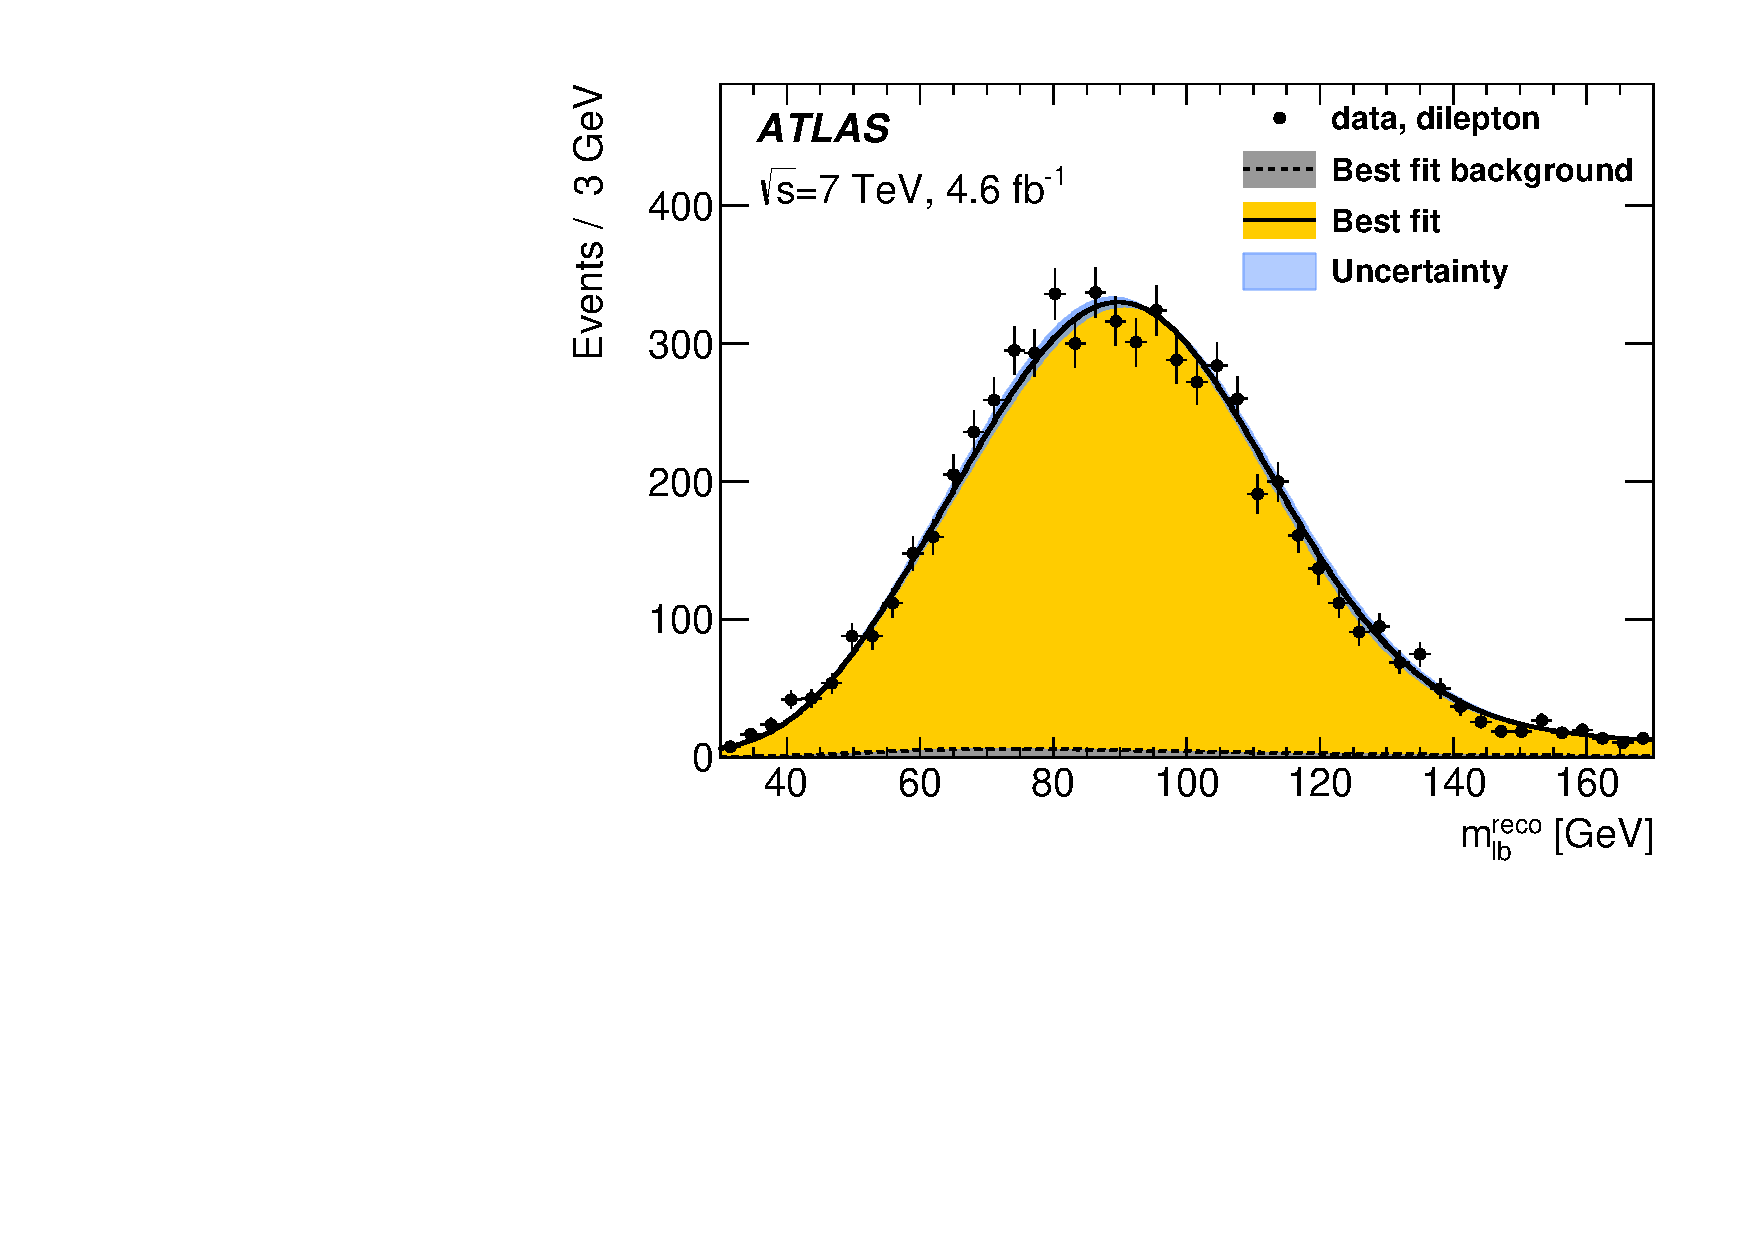
\includegraphics[height=0.37\textwidth]{figs/Fit_data_rlbcalo_mlb_ele2_4600invpb.pdf}
	\label{sfig:mlbrecofit}
}
\subfloat[\mt\ likelihood profile]{
	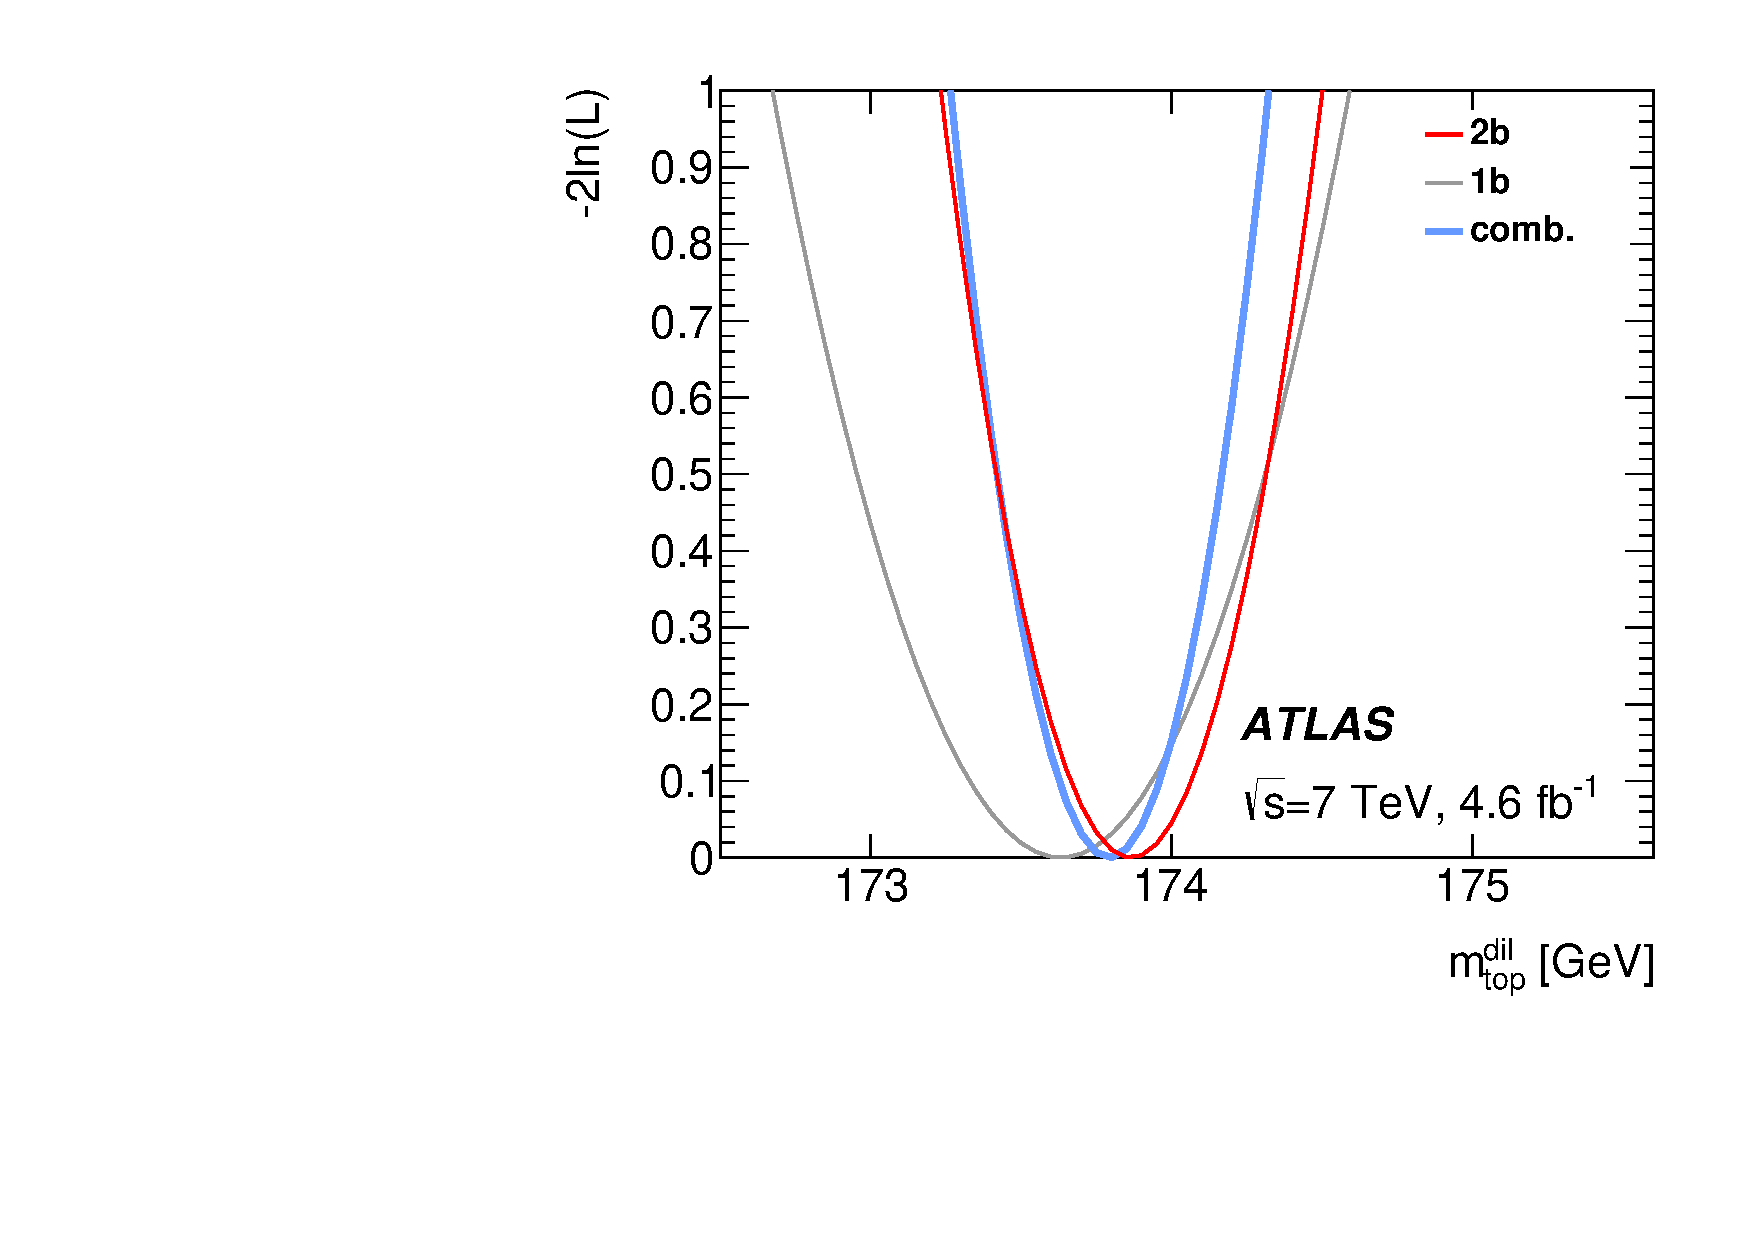
\includegraphics[height=0.37\textwidth]{figs/Compare_1and2btag_results_3.pdf}
	\label{sfig:llmtoplike}
}
%
\caption[Likelihood fit for $\sqrts=7$~\TeV\ data]{
%
\Fig~\subref{sfig:mlbrecofit} shows the data distribution for one and two \btagged\ jets of \mlbr\ and the fitted \glspl{pdf} for the background alone and for signal-plus-background, using an unbinned likelihood fit. 
%
The uncertainty band indicates the total uncertainty on the signal-plus-background fit obtained from pseudo-experiments as explained in the text. 
%
\Fig~\subref{sfig:llmtoplike} shows the likelihood profile as a function of \mt, denoted by \mtdl\ in the figure, for the sample with one \btagged\ jet (grey), the sample with two \btagged\ jets (red) and the combined result (blue). 
%
\label{fig:results7TeV}}
\end{figure*}
%%%%%%%%%%%%%%%%%%%%%%%%%%%%%%%%%%%%%%%%%%%%%%%%%%%%%%%%%%%%%%%%%%%%%%%%%%%%%
%


















\section{Uncertainties affecting the \mt determination}
\label{sect:unc7TeV}
%
% Uncertainties on the measurement of a physics observable comprise both statistical or systematic effects. 
%
While the statistical uncertainties are determined from the likelihood maximisation, this section focusses on the treatment of uncertainty sources of systematic nature.
%
%
Several sources of systematic uncertainties are considered. 
%
Their impact on the analysis is mostly evaluated by varying the respective quantities by $\pm 1 \sigma$ with respect to their default values, constructing the corresponding template and measuring the average \mt change  with respect to the result from the nominal \gls{MC} sample with $500$ pseudo-experiments each, drawn from the full \gls{MC} sample. 
%
Half this \mt change, corresponding to one standard deviation, is then quoted as systematic uncertainty from this source, if not stated otherwise. 
%
In view of a combination with results from the \ttbarlj\ channel, every systematic uncertainty is assigned a statistical uncertainty, taking into account the statistical correlation of the considered samples. 
%
The resulting total uncertainty and all components are listed in \tab~\ref{tab:llresults7TeV}, irrespective of their statistical significance. 
%
This approach follows the suggestion in \reference~\cite{Barlow:2002yb} and relies on the fact that, given a large enough number of considered uncertainty sources, statistical fluctuations wash out. 
%
The uncertainty sources are constructed to be used uncorrelated between each other and thus the total uncertainty is calculated as the sum in quadrature of all components. 
%
The various sources of systematic uncertainties and their evaluation are described in the following.
%






%--------------------------------------------------------------------------
\subsection{Statistics and method calibration}
%
Uncertainties related to statistical effects or method calibration are discussed here.
%
%
\paragraph{Statistics}\mbox{}
%
The statistical uncertainty on the \mt\ determination is taken from the symmetrised \mt\ values corresponding to the likelihood values at $-2\ln{\Like^\mathrm{min}} + 1$, displayed in \fig~\subref*{sfig:llmtoplike}. 
%
\paragraph{Method}\mbox{}
%
The residual difference in fitted and underlying \mt\ when analysing a template from an \gls{MC} sample reflects the bias of the method. 
%
The largest average difference observed in pseudo-experiments for the samples with different \mt\ values is quoted as uncertainty. 
%
This uncertainty also covers effects from limited \gls{MC} statistics in the templates.



%
%--------------------------------------------------------------------------
\begin{table*}[tb!]
%\footnotesize
\small
\begin{center}
\begin{tabular}{|l|r|}\cline{2-2}
\multicolumn{1}{c|}{}         &  \mt\ [\GeV]      \\ \hline
            Result            &  173.79           \\ \hline
        Statistics            &    0.54           \\ \hline
            Method            & 0.09 $\pm$ 0.07   \\
Signal \glsdesc{MC} generator & 0.26 $\pm$ 0.16   \\
     Hadronisation            & 0.53 $\pm$ 0.09   \\
  \glsdesc{ISRFSR}            & 0.47 $\pm$ 0.05   \\
      \glsdesc{UE}            & 0.05 $\pm$ 0.05   \\
      \glsdesc{CR}            & 0.14 $\pm$ 0.05   \\
     \glsdesc{PDF}            & 0.11 $\pm$ 0.00   \\ \hline
   $W/Z$+jets normalisation   & 0.01 $\pm$ 0.00   \\
  $W/Z$+jets shape            & 0.00 $\pm$ 0.00   \\
       \fake normalisation    & 0.04 $\pm$ 0.00   \\
       \fake shape            & 0.01 $\pm$ 0.00   \\ \hline
     \glsdesc{JES}            & 0.75 $\pm$ 0.08   \\
    \Glsdesc{bJES}            & 0.68 $\pm$ 0.02   \\
     \glsdesc{JER}            & 0.19 $\pm$ 0.04   \\
     \glsdesc{JRE}            & 0.07 $\pm$ 0.00   \\
     \glsdesc{JVF}            & 0.00 $\pm$ 0.00   \\
             \btag            & 0.07 $\pm$ 0.00   \\
           Leptons            & 0.13 $\pm$ 0.00   \\
              \met            & 0.04 $\pm$ 0.03   \\
           Pile-up            & 0.01 $\pm$ 0.00   \\ \hline
 Total systematics            & 1.31 $\pm$ 0.23   \\ \hline
             Total            & 1.41 $\pm$ 0.24   \\ \hline
\end{tabular}
\end{center}
\caption[Systematic uncertainties on \mt\ for $\sqrts=7$~\TeV\ data]{
%
The measured value of \mt together with the statistical and systematic uncertainty components for the $\sqrts=7$~\TeV\ data. 
%
Values quoted as 0.00 are smaller than 0.005. 
%
The last line gives the sum in quadrature of the statistical and systematic uncertainty components. 
%
\label{tab:llresults7TeV}}
\end{table*}
%--------------------------------------------------------------------------





%--------------------------------------------------------------------------
\subsection[Modelling of \texorpdfstring{$\ttbar$}{ttbar} processes]{Modelling of \texorpdfstring{\boldmath$\ttbar$}{ttbar} processes}



\label{sect:systtbarmod7TeV}
%
\Tquark\ pair processes have a rich physics environment and are consequently subject to various systematic effects, ranging from the \ttbar\ production to the hadronisation of the showered objects. The corresponding uncertainties are discussed here.
%
%
\paragraph{Signal \glsdesc{MC} generator}\mbox{}
%
The impact of the choice of the \ttbar\ signal \gls{MC} generator is determined by comparing an event sample produced with \Mcatnlo~\cite{FRI-0201,FRI-0301} to the default \Powheg\ sample, both generated at $\mt=172.5$~\GeV\ and using the \Herwig\ program for the hadronisation.
%
The full observed difference is quoted as systematic uncertainty.
%
This approach follows the observation that \Mcatnlo\ and \Powheg\ samples exhibit jet multiplicities for the \ttbarlj\ channel, which bracket those observed in the data~\cite{ATLASCollaboration2015}.
%
The generator \Alpgen\ was not used for this comparison due to possible distortions in the estimator distributions caused by the unphysical treatment of the \tquark\ and \Wboson\ decay width within this program~\cite{ATL-PHYS-INT-2014-001}. 
%
In addition, the impact of variations of the factorisation and renormalisation scales ($\mu_{\mathrm{F/R}}$) was determined within \Powheg\ to be $0.14\pm 0.05~\GeV$. 
%
Within statistical uncertainties, this value is consistent with the differences observed from the \Mcatnlo\ and \Powheg comparison and therefore assumed to be already covered.
%  
%  
\paragraph{Hadronisation}\mbox{}
%
To cover the choice of the hadronisation model, samples produced with the \Powheg\ event generator are processed with either \Pythia\ using the P2011C tune or \Herwig\ and \Jimmy\ using the ATLAS AUET2 tune~\cite{ATL-PHYS-PUB-2011-008}.
%
This includes different approaches in shower modelling, like the usage of a \pt\ or angular ordered \gls{PS}, \gls{PS} matching scales, fragmentation functions and hadronisation models like the choice of the Lund--String model~\cite{Andersson198331,Andersson:1998tv}, implemented in \Pythia, or the cluster fragmentation model~\cite{Webber:1983if} used in \Herwig. 
%
The full observed difference of the samples is quoted as systematic uncertainty. 
%
Due to a $\tau$~lepton polarisation modelling problem in the \PowhegHerwig\ sample, events containing $W\to \tau\nu$ decays were excluded from the evaluation. The effect is expected to be negligible, since the difference is purely leptonic and has no effect on the colour charge topology, whose modelling stability is assessed in this systematic uncertainty. 



The calibration of the \gls{JES} and \gls{bJES}, which is discussed in detail below, is also partially based on a comparison of jet energy responses in \Herwigpp\ and \Pythia\ event samples.
%
The jet energy response is defined as the ratio of \recolevel\ to \stablevel\ jet \pt, referred to as \truelevel\ in this context, $\resp=\pt^\mathrm{reco}/\pt^\mathrm{truth}$. The response typically ranges from 0.5 to 0.9, due to energy loss effects like out-of-cone radiation dominanting over gain effects like pile-up.
%
Despite the fact that the \gls{JES} and \gls{bJES} is estimated independently using dijet and other non-\ttbar\ samples~\cite{ATLASCollaboration2015b}, a certain level of double-counting of uncertainty components cannot be excluded. 
%
This has been investigated closely for the \gls{ATLAS} \tquark\ mass measurement in the \ljets\ channel~\cite{Aad:2015nba} by a recalibration of the jets in a \Pythia\ sample to match the jet response observed in \Herwig, thus eliminating the double-counting from jet energy response differences~\cite{ATL-PHYS-PUB-2015-042}. 
%
This has been performed in two ways: jet flavour inclusively, removing the effect for the \gls{JES}, and flavour-by-flavour, using a minimum \dR\ parton to jet matching, which removes the \gls{bJES} double-counting.
%
A fit within the framework of the analysis yields no significant change in the difference of fitted masses of \PowhegPythia\ and, consequently, the amount of double-counting of \gls{JES} and hadronisation effects for the \ljets\ channel is small. 
%
A similar behaviour is expected for the \dil\ channel.
%
%
\glsreset{ISRFSR}
\paragraph{\gls{ISRFSR}}\mbox{}
%
\gls{ISRFSR} leads to a higher jet multiplicity and different jet energies in the event, which affects the estimator distributions. 
%
The effect is evaluated by comparing two dedicated samples generated with \Acermc~\cite{SAMPLES-ACER} in combination with \Pythia\ P2011C for hadronisation and the \gls{PS}. 
%
In each of those, the \Pythia\ P2011C tune is replaced by other tunes with different values of \alphas\ used in the \gls{PS}, relevant for the amount of \gls{ISRFSR}. The variations are performed in ranges according to a study of additional jets in \ttbar\ events~\cite{ATL-2012-033}. 
%
Half the observed difference is quoted as systematic uncertainty.
%
%
\glsreset{UE}
\paragraph{\gls{UE}}\mbox{}
%
The systematic uncertainty connected with the \gls{UE} is estimated using samples simulated with \Powheg-hvq and \Pythia, which are based on the same \genlevel\ \Powheg-hvq events generated with the CT10 \glspl{PDF}. 
%
The difference in \gls{UE} modelling is assessed by comparing a sample with the Perugia 2012 tune (P2012) to a sample with the P2012 mpiHi tune~\cite{Skands}, with both tunes using the same CTEQ6L1 \glspl{PDF}~\cite{cteq5l} for \gls{PS} and hadronisation. The Perugia 2012 mpiHi tune provides more semi-hard multiple parton interactions and is used for this comparison with identical \gls{CR} parameters in both tunes. The full observed difference is assigned as systematic uncertainty. 
%
%
%This was just requested info for the paper
% The mpiHi tune introduces more semi-hard multiple parton interactions, but it yields similar predictions for an observable sensitive to the \gls{UE} activity in inclusive \pp\ collisions~\cite{ATL-PHYS-PUB-2011-009}, the activity in the transverse plane of the leading \pt\ charged particle. The \gls{CR} tunes, to be discussed next, produce notably different predictions and cover variations in this observable. \todo{why evaluate UE with tunes that leave UE sensitive observables unchanged??}
%
%
\glsreset{CR}
\paragraph{\gls{CR}}\mbox{}
\gls{CR} denotes the strong interaction between colour singlet parton systems originating at different stages of the event evolution. It influences the development of the \gls{PS} and the subsequent hadronisation. The strength of \gls{CR} effects in simulation is tuned to match the observation in data.
%
The systematic uncertainty connected with the \gls{CR} is estimated using the same samples as the ones for \gls{UE}, but with the P2012 tune and the P2012 loCR tune~\cite{Skands} for \gls{PS} and hadronisation. 
%
The \gls{CR} effects are estimated by assigning the full difference observed between samples. 
%
%This was just requested info for the paper
% As measured in \reference~\cite{ATL-PHYS-PUB-2011-009}, the P2012 loCR tune leads to significantly less activity in the transverse region of the leading \pt\ charged particle than the standard P2012 tune.
% %
% Therefore, the observed differences also cover the uncertainty associated with the particle spectra in the \gls{UE}.
%
%
\paragraph{\acrlong{PDF} (\acrshort{PDF})}\mbox{}
%
\glspl{PDF} are determined from a global fit to short distance scattering data. Therefore, they have an experimental uncertainty, which is reflected in this case in 26~pairs of independent \gls{PDF} variations provided by the CTEQ group~\cite{Pumplin2002}.
%
The uncertainty based on the CT10 set is evaluated by pairwise comparison of templates, produced with reweighted events according to each of the 26 \gls{PDF} variations, and assigning half of the observed difference as uncertainty. 
%
The final uncertainty is obtained by summing up the single components in quadrature and amounts to 0.10~\GeV.
%
Additionally, a reweighting comparison of the central CT10 \gls{PDF} set to two independently evaluated \gls{PDF} sets is performed, namely to the MSTW2008~\cite{MAR-0901} and the NNPDF23~\cite{Ball:2012cx} \glspl{PDF}. 
%
The corresponding differences amount both to 0.01~\GeV.
%
The final \gls{PDF} systematic uncertainty is the sum in quadrature of these three contributions.
%







%--------------------------------------------------------------------------
% \subsection{Modelling of non-\texorpdfstring{\ttbar}{ttbar} processes}
\subsection[Modelling of non-\texorpdfstring{$\ttbar$}{ttbar} processes]{Modelling of non-\texorpdfstring{\boldmath$\ttbar$}{ttbar} processes}
%
The contribution of non-\ttbar\ processes is very low, thanks to the restrictive selection requirements. 
%
Nevertheless mismodelling of these processes is taken into account by variation of the corresponding normalisations and distribution shapes.
%
%
\paragraph{$W/Z$+jets normalisation and shape} 
%
The \Wj\ background normalisation uncertainty is dominated by the uncertainty on the heavy-flavour content, as shown in \reference~\cite{CERN-PH-EP-2012-015} and the same normalisation uncertainty is assigned to the \Zj\ background.
%
The overall uncertainty for both kinds of processes amounts to $\pm30\%$.
%
The $\Wbos/\Zbos$ boson event shape uncertainty covers variations of \Alpgen\ parameters and the parton shower matching scale.
%
Due to the vanishing contribution of the \Wj\ background, the corresponding uncertainties have no impact on the analysis. 
%
%
\paragraph{\fake\ normalisation and shape} 
%
The uncertainty connected to the \fake\ background normalisation following the matrix method is $\pm50\%$~\cite{Aad:2010ey}. 
%
Shape variations arising from efficiency variations of the real and fake leptons are evaluated and added in quadrature. 
%
Additionally, for the fake muon background, two independent matrix methods are applied, and their difference is taken as systematic uncertainty and added in quadrature. 
%
Detailed information on the determination of \fake\ background can be found in \reference~\cite{ATLAS-CONF-2014-058}. 
%
%
\paragraph{Single \tquark\ contribution} 
%
The single \tquark\ normalisation uncertainties are estimated from the corresponding uncertainty on the theoretical cross sections. 
%
The resulting systematic uncertainty is negligible.










%--------------------------------------------------------------------------
\subsection{Detector modelling} 
\label{sect:detectormodelling7TeV}
%
The limited knowledge of the detector and the particle interactions therein is reflected in numerous systematic uncertainties.
%
%
\glsreset{JES}
\paragraph{\gls{JES}}\mbox{}
%
The \gls{JES} is derived from test-beam data, \gls{LHC} collision data and simulation. If unconstrained, its uncertainties dominantly limit the precision of \tquark\ mass measurements at hadron colliders. 
% 
Jet energies can be measured with a relative precision of about $1\%$ to $4\%$, typically falling with jet \pt\ and rising with jet $\eta$~\cite{ATLASCollaboration2015b}. This is shown as a function of \pt\ in \fig~\ref{fig:JES7TeV}. 
%
%
% %%%%%%%%%%%%%%%%%%%%%%%%%%%%%%%%%%%%%%%%%%%%%%%%%%%%%%%%%%%%%%%%%%%%%%%%%%%%%%%
% \begin{figure*}[tbp!]
% \centering
% \subfloat[\gls{JES} uncertainty for \ljet{s}]{
% 	\includegraphics[width=0.49\textwidth]{./figs/JES_7TeV_EMJES_61a.pdf}
% 	\label{sfig:lightJES7TeV}
% }
% \subfloat[\gls{JES} uncertainty for \bjet{s}]{
% 	\includegraphics[width=0.49\textwidth]{figs/bJES_7TeV_EMJES_65a.pdf}
% 	\label{sfig:bJES7TeV}
% }
% \caption[\gls{JES} uncertainties for $\sqrts=7$~\TeV\ data]{
% %
% The sample-dependent fractional \gls{JES} uncertainty for jets in \semileptonic\ \tquark\ pair decays with at least two \btagged\ jets as a function of \pt\ \subref{sfig:lightJES7TeV} for \ljet{s} and \subref{sfig:bJES7TeV} for \bjet{s} with the average 2011 pile-up conditions~\cite{ATLASCollaboration2015b}. The exact values are analysis dependent and do not necessarily match the shown curves exactly.
% %https://atlas.web.cern.ch/Atlas/GROUPS/PHYSICS/PAPERS/PERF-2012-01/
% %
% \label{fig:JES7TeV}
% }
% \end{figure*}
% %%%%%%%%%%%%%%%%%%%%%%%%%%%%%%%%%%%%%%%%%%%%%%%%%%%%%%%%%%%%%%%%%%%%%%%%%%%%%
% %
%
%%%%%%%%%%%%%%%%%%%%%%%%%%%%%%%%%%%%%%%%%%%%%%%%%%%%%%%%%%%%%%%%%%%%%%%%%%%%%%%
\begin{figure*}[tbp!]
\centering
\subfloat[\gls{JES} uncertainties as a function of the jet \pt]{
	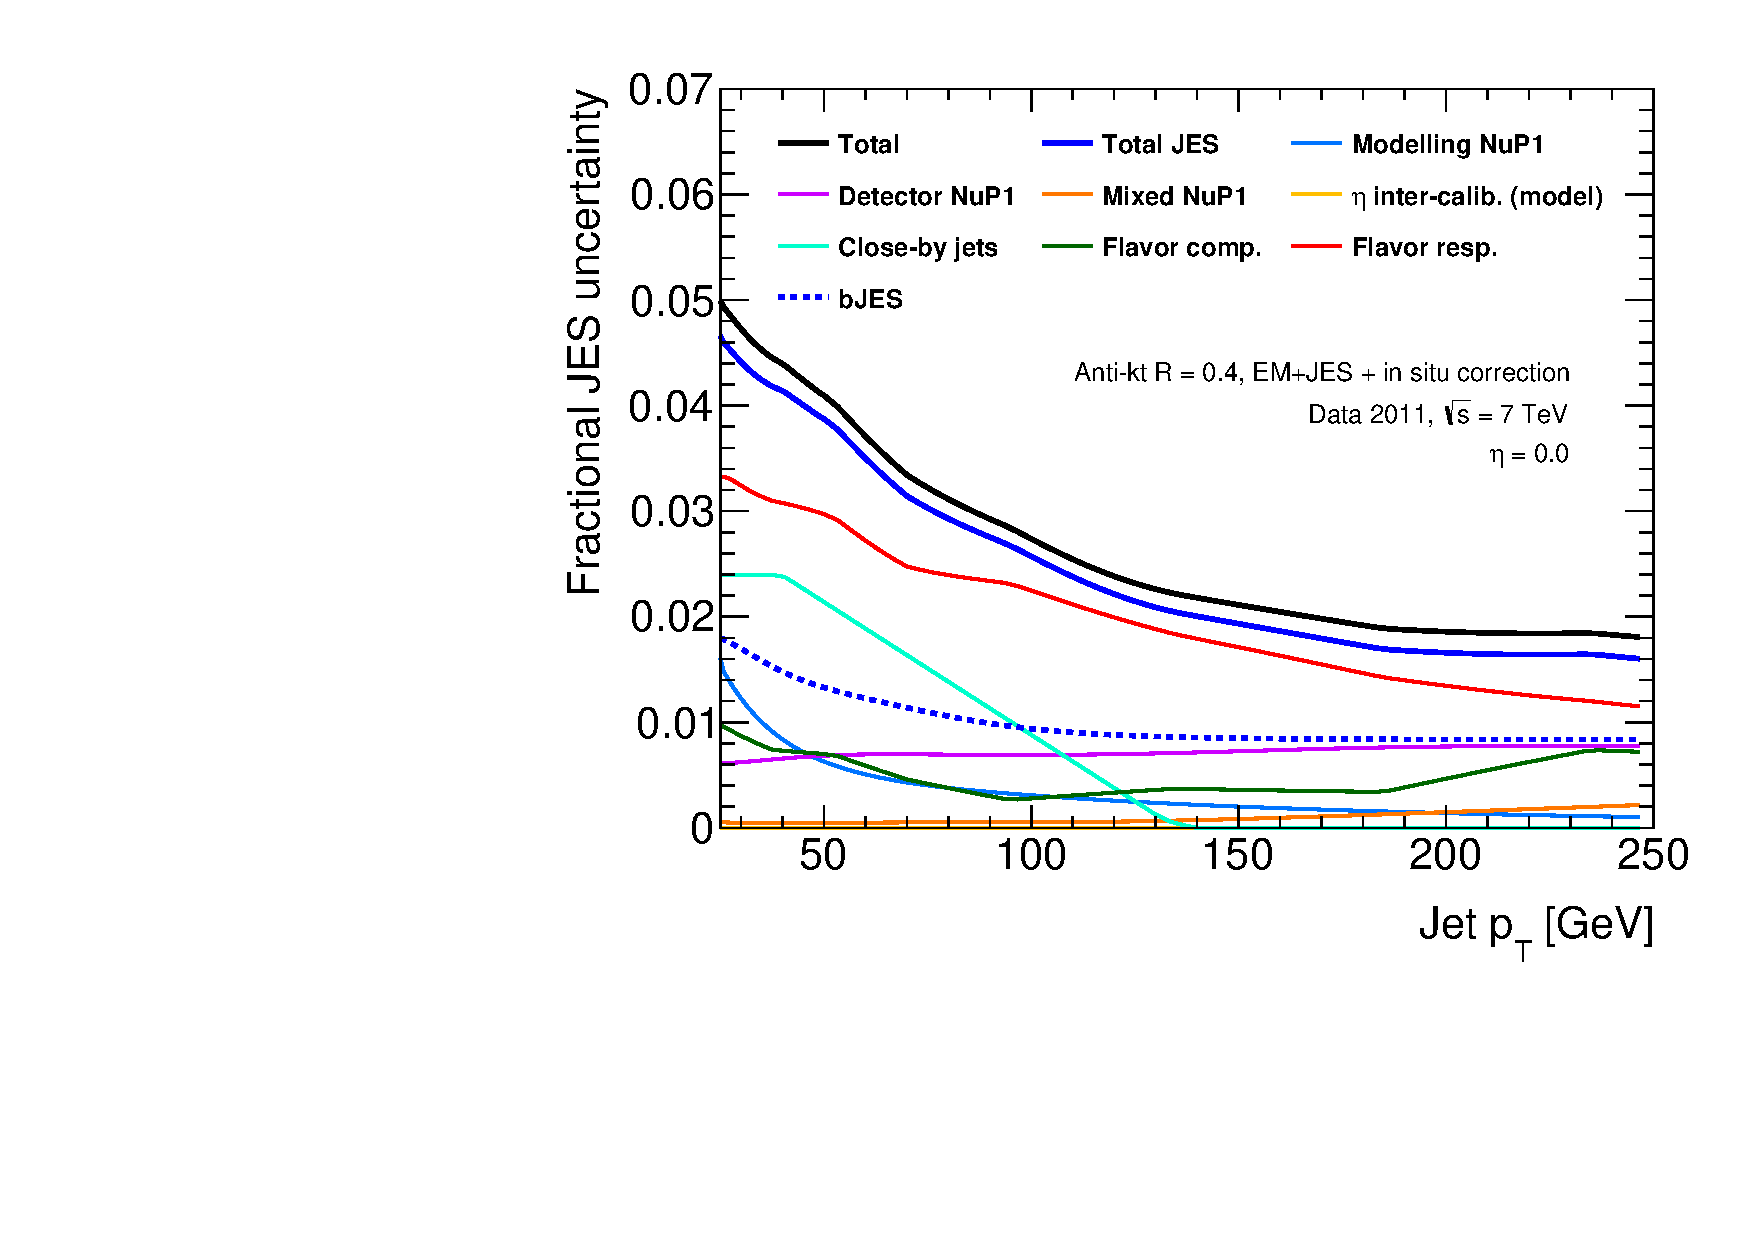
\includegraphics[width=0.49\textwidth]{./figs/fig_8TeV_TRC28_wp70//PlotJESUncertaintyComponents_Final17_TRC28_7TeV_0.pdf}
	\label{sfig:JES7TeVpt}
}
\subfloat[\gls{JES} uncertainties as a function of the jet $\eta$]{
	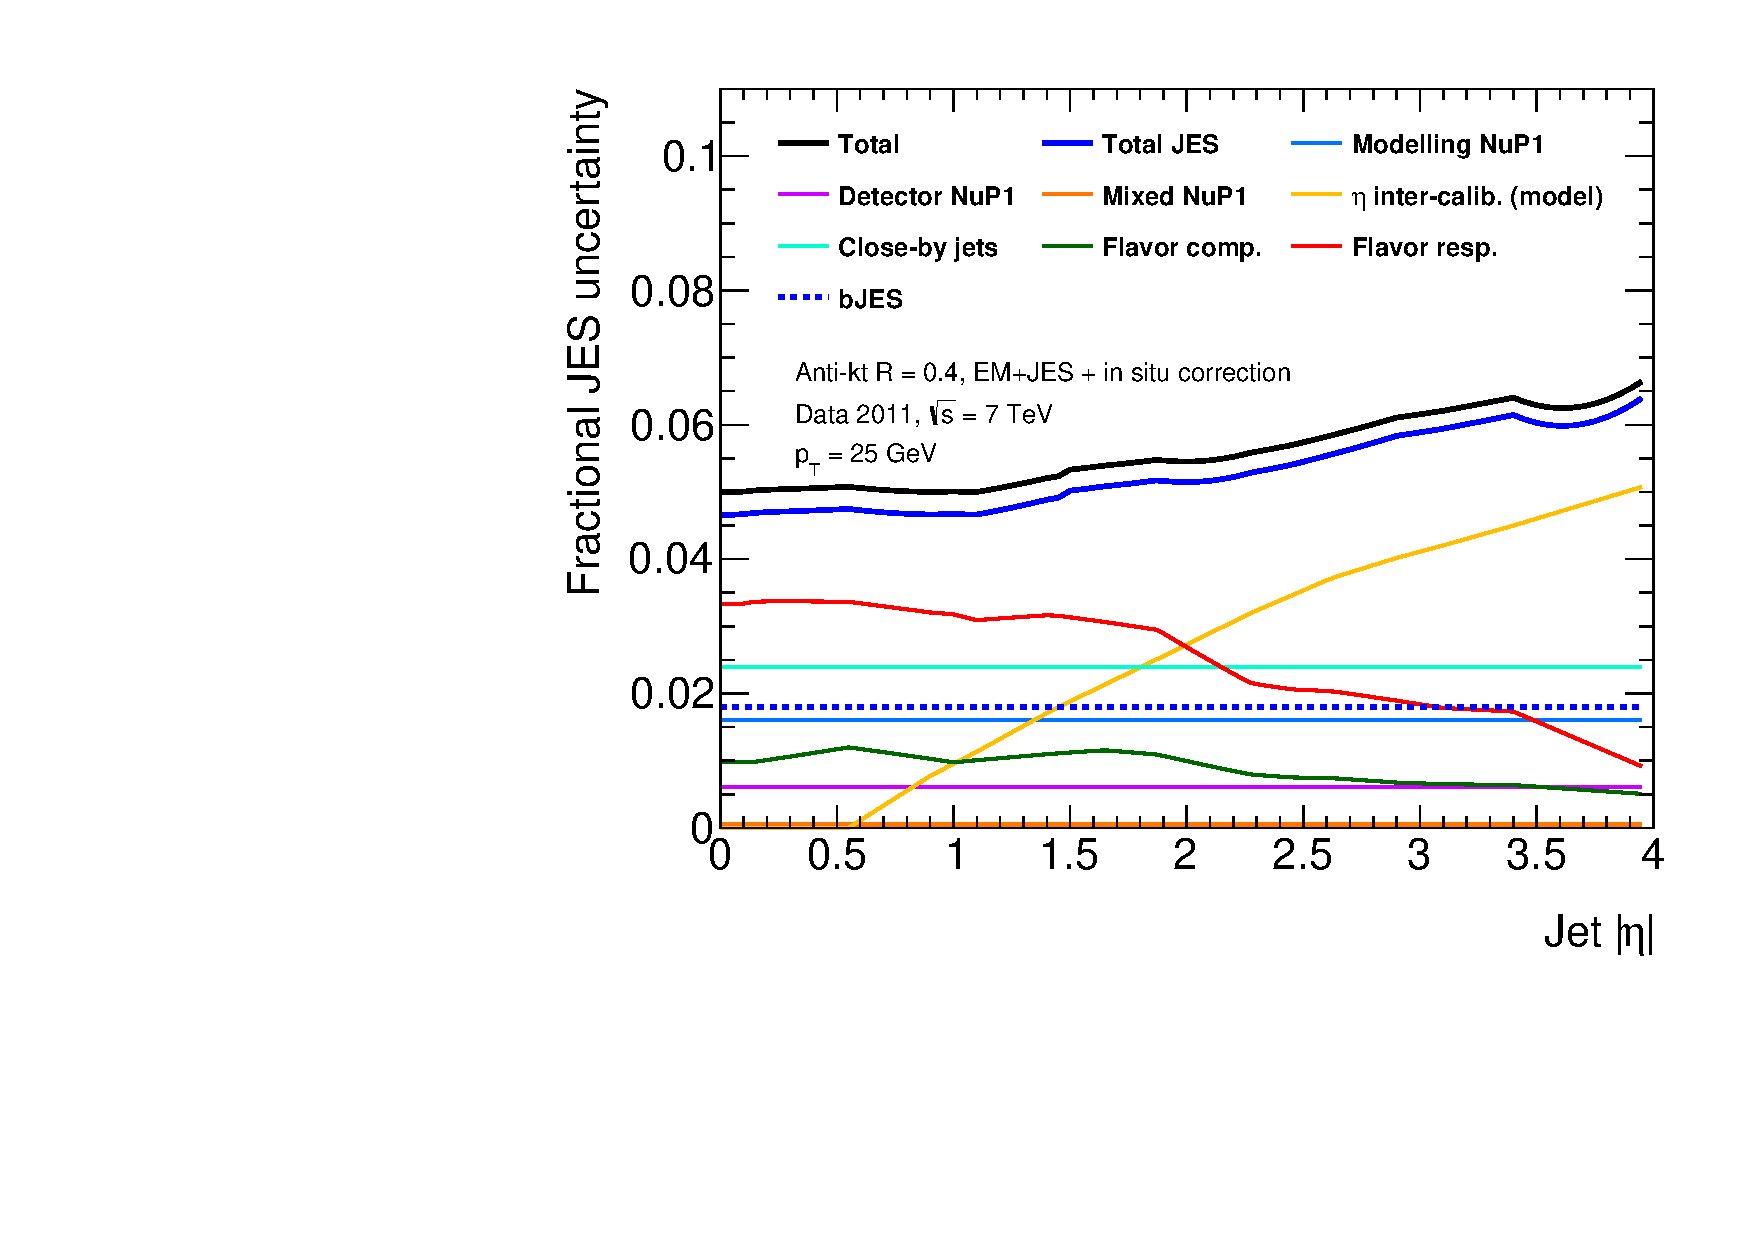
\includegraphics[width=0.49\textwidth]{figs//fig_8TeV_TRC28_wp70/PlotJESUncertaintyComponents_Final17_TRC28_7TeV_3.pdf}
	\label{sfig:JES7TeVeta}
}
\caption[\gls{JES} uncertainties for $\sqrts=7$~\TeV\ data]{
%
The fractional \gls{JES} uncertainty for jets at $\sqrts=7$~\TeV\ as a function of jet \pt~\subref{sfig:JES7TeVpt} and $\eta$~\subref{sfig:JES7TeVeta}. 
%
The most significant components in terms of systematic uncertainty on the \mt\ measurement and the flavour related uncertainties using the \dil\ \gls{QGF} information are shown as well.
%
The values correspond to events with three jets and the respective pile-up conditions in 2012 data. The average values for the analyses are selection dependent and do not necessarily match the shown curves exactly.
%
\label{fig:JES7TeV}
}
\end{figure*}
%%%%%%%%%%%%%%%%%%%%%%%%%%%%%%%%%%%%%%%%%%%%%%%%%%%%%%%%%%%%%%%%%%%%%%%%%%%%%
%
The total \gls{JES} uncertainty consists of more than 60 subcomponents, originating from the various steps in the jet calibration. 
%
The components are classified in the categories `Statistical', `Detector', `Modeling', `Mixed', or `Special'. This comprises statistical components from in-situ calibration, detector related components like energy scales and resolutions of \gls{EM} objects and modelling components for \Gammaj\ and \Zj\ calibration. In addition, the uncertainty related to the intercalibration for phase space regions in $\eta$ or \pt, which are not accessible with the standard calibration approaches, is taken into account. Also, uncertainties related to the flavour composition of the event and the correction for pile-up or close-by jets are considered. 
%
The number of these \gls{NuP} can be significantly reduced with a matrix diagonalisation of the full \gls{JES} covariance matrix, including all \gls{NuP} of a given category of the \gls{JES} uncertainty components. 
%
This approach preserves the correlations of the uncertainties in different phase space regions with 10\% accuracy. 
%
Variations with negligible eigenvalues are dropped, leading to a significant reduction in complexity~\cite{ATLASCollaboration2015b}. 
%
Here, a reduced set of 21 uncorrelated \pt- and $\eta$-dependent parameters is used.
%
The individual components of the reduced set grouped by category are given in \tab~\ref{tab:jesresults7TeV} in \chap~\ref{chap:combinations}. 
%
For the flavour composition and response uncertainties, the analysis-specific \gls{QGF} has been determined, leading to an improvement of the final precision by \order(20)~\MeV. This is detailed in \sect~\ref{sect:qgf7TeV}. 
%
The dominant \gls{JES} uncertainty components stem from the $\eta$ inter-calibration modelling and the leading \gls{NuP} of the detector category. The \gls{JES} uncertainty is the dominant uncertainty contribution for this analysis. 

%
%
%
\glsreset{bJES}
\paragraph{\Gls{bJES}}\mbox{}
%
The \gls{bJES} is an additional uncertainty for the remaining differences of \bjet{s}\ and \ljet{s} after the global \gls{JES} has been applied and therefore the corresponding uncertainty is uncorrelated with the \gls{JES} uncertainty. 
%
Jets originating from a \bhadron\ are assigned an additional uncertainty of $0.7\%$ to $1.8\%$, with lowest uncertainties for high-\pt\ \bjet{s}. The \gls{bJES} is shown in \fig~\ref{fig:JES7TeV} as a function of jet \pt\ and $\eta$. 
%
The \gls{bJES} uncertainty is obtained from \gls{MC} simulation and verified in the data. 
%
The validation is performed by comparison of \btagged\ calorimeter jets with the corresponding track jets, consisting of charged particles measured in the \gls{ID}.
%
Different \gls{MC} models were used to study \bquark\ fragmentation, hadronisation and underlying soft radiation~\cite{ATLASCollaboration2015b}. 
%
In the \ttbarll\ channel, the \gls{bJES} uncertainty is the second largest contribution. 
%
%- Info on bJes uncertainty: https://atlas.web.cern.ch/Atlas/GROUPS/PHYSICS/PAPERS/PERF-2012-01/fig_53b.png
%
\glsreset{JER}
\paragraph{\gls{JER}}\mbox{}
%
Jet reconstruction suffers from limited jet energy resolution, which is not perfectly modelled in \gls{MC}. 
%
The residual difference of \gls{MC} and data can be mimicked by applying a random Gaussian shift on the jet energies before event selection, such that the final width of the response distribution equals the one observed in data~\cite{Aad:1489592}. 
%
The fitted \mt\ difference of the varied sample to the nominal sample is taken as uncertainty.
%
%
\glsreset{JRE}
\paragraph{\gls{JRE}}\mbox{}
%
The \gls{JRE} is the efficiency to reconstruct a jet in the calorimeter, rising from about 95\% for jets with $\pt=25$~\GeV\ to full efficiency above $\pt=30$~\GeV.
%
The \gls{JRE} in the data and \gls{MC} is found to agree within $2\%$ and less than $1\%$ for jets below and above $\pt=30$~\GeV, respectively~\cite{Aad:1409965}. 
%
These residual differences are accounted for by randomly removing $2\%$ of the jets with $\pt< 30$~\GeV\ from the events prior to the event selection. 
%
The fitted \mt\ difference of the varied sample to the nominal sample is taken as uncertainty.
%
%
\glsreset{JVF}
\paragraph{\gls{JVF}}\mbox{}
% 
The fraction of jet tracks associated to the primary vertex is used for pile-up suppression. 
%
Its modelling shows differences to the data and a correction using jet \pt\ dependent scale factors is applied. 
%
The corresponding uncertainty is evaluated by variation of the scale factors within their uncertainties and turns out to be small.
%
%
\paragraph{\boldmath$\btag$}\mbox{}
%
Mismodelling of the \btag\ efficiency and mistag rate is accounted for by the application of jet specific scale factors to \gls{MC} events~\cite{Aad:2015ydr}.
%
These scale factors depend on the jet \pt\ and $\eta$ and the underlying quark flavour. 
%
The ones used in this analysis were derived from dijet and \ttbarll~\cite{Aad:2015ydr} events. 
%
Since the \btag\ scale factor determination is systematically limited, the statistical correlation, induced by the use of the \ttbarll\ scale factors in the same channel they were derived in, is estimated to be negligible. 
%
Systematic uncertainties that are common in the analysis and the \btag\ calibration are treated in a correlated way. To properly treat these uncertainties, their contribution is subtracted from the \btag\ scale factor covariance matrix, and the varied \btag\ scale factors are instead applied to the events when evaluating the common systematic uncertainty at the \mt\ analysis level.
%
The uncertainty on the correction factors is split into ten uncorrelated components. 
%
Their impact is derived by variation of the scale factors within their uncertainties and adding the resulting fitted differences in quadrature. 
%
A similar procedure is applied for the four components of the scale factors corresponding to \cjet{s}. 
%
Additionally, the scale factors for \ljet{s} are varied within their uncertainties. The final \btag\ uncertainty is the sum in quadrature of these uncorrelated components.
%
%
\paragraph{Lepton uncertainties}\mbox{}
%
The lepton uncertainties are related to the electron energy or muon momentum scale, resolution and identification efficiencies. 
%
These have been measured very precisely in high purity $Z\to \ell\ell$ data~\cite{CERN-PH-EP-2014-040,
CERN-PH-EP-2014-151}.
%
The corresponding uncertainty is propagated to the analysis by variation of the respective quantity. The changes are propagated to the \met\ as well. 
%
%
\paragraph{Missing transverse momentum (\boldmath$\met$)}\mbox{}
%
The \met\ is constructed as the negative sum of all measured particle \pt\ and \et\ in the detector.
%
Consequently, a miscalibration of any of these components has a direct impact in the \met\ calculation. 
%
For reconstructed objects, this effect is covered by a recalculation of the \met. 
%
The uncertainties in calorimeter cell energies associated with low-\pt\ jets ($7~\GeV< \pt < 20~\GeV$), without any corresponding reconstructed physics object or from pile-up interactions, are accounted for in this dedicated \met\ uncertainty~\cite{ATLAS-MET-NEW}.
%
Since the \met\ is merely used for the event selection, the corresponding uncertainty is small.
%
%
\paragraph{Pile-up}\mbox{}
%
Besides the component treated in the \gls{JES} uncertainty, the residual dependence of the fitted \mt\ on the amount of pile-up activity has been determined in the data and simulation as functions of \nvtx\ and \meanmu. 
%
The slope of the linear dependence observed in simulation on the \mt\ measurement amounts to $0.15\pm0.02$~\GeV\ per vertex and $0.11\pm0.03$~\GeV\ per interaction, with the uncertainties being of statistical nature only. This observation is consistent in the data and \gls{MC}.
%
The final effect on the measurement is assessed by a convolution of the linear dependence with the respective \nvtx\ and \meanmu\ distributions observed in the data and \gls{MC}. 
%
The maximum of the \nvtx\ and \meanmu\ effects is assigned as uncertainty due to pile-up.









\subsection{Statistical precision of systematic uncertainties}
\label{sect:syststat}
%
The systematic uncertainties quoted in \tab~\ref{tab:llresults7TeV} carry statistical uncertainties themselves. In view of a combination with other measurements, the statistical precision from a comparison of two samples $\sigma_{12}$ is determined for each uncertainty source based on the correlation $\rho_{12}$ of the underlying samples, following $\sigma_{12}^2=\sigma_1^2+\sigma_2^2-\rho_{12}\sigma_1\sigma_2$. The correlation is usually expressed as a function of the fraction of shared events of both samples $\rho_{12}=\sqrt{\N{12}/((\N{1}+\N{2})/2)}$, with $\N{1/2}$ being the number of events in the respective sample. An alternative way, using a set of pseudo-experiments to randomly draw events from the union of both samples and assess their correlation, produces similar results and is not used for simplicity. 
%
The \gls{MC} samples used here have an integrated luminosity in the range $\intlumi=100$ to $300~\invfb$ and the statistical precision on a single sample fit ranges from about $65$ to $110$~\MeV. 
%
Most estimations are based on the same sample with only a change in a single parameter, leading to a high correlation of the central \mt\ values and a correspondingly low statistical uncertainty on their difference. 
%
Others, which do not share the same generated events or exhibit other significant differences, have a lower correlation and the corresponding uncertainty is higher, like in the case of the signal \gls{MC} modelling uncertainty. Due to the relatively low precision, the determination of this uncertainty component would especially profit from higher \gls{MC} statistics.

%Giorgio says, too detailed:
% The signal \gls{MC} generator uncertainty is evaluated from two disjunct generators for the hard scattering event. The samples are statistically uncorrelated and the precision of the difference is therefore simply the sum in quadrature of the individual uncertainties. 
% %
% This is not the case for the Hadronisation, the \gls{UE}, the \gls{CR} and the \gls{ISRFSR} sources, which share the generated hard scattering events. Due to details of the \gls{ATLAS} simulation procedure, a one-to-one matching of events with the same underlying hard scattering and consequently an exact determination of the sample overlap is not possible. Therefore, a 50\% overlap of the samples is assumed, corresponding to a 71\% statistical correlation to be used for the uncertainty determination. 
% %
% The systematic uncertainty sources whose impact is assessed based on the variation of scale factors share the same events and have 100\% overlap. Consequently, the \btag, the lepton trigger, reconstruction and identification and the \gls{PDF} uncertainties have negligible statistical uncertainty. 
% %
% The precision of the composite \gls{JES} uncertainty is evaluated, using the correlation of the different up and down variations, which is typically $\order(99\%)$ due to the high overlap of the varied samples. Consequently, the final statistical precision is only insignificantly larger than the precision for a single sample measurement. 
%
% \todo{which JER correlation assumed for dilepton? 92 or lower because of ljets arguments? INTNOTE}
% An exception to the above methodology has however to be made for the Jet Energy
% Resolution systematics. In this case the fraction of common events of the
% default and varied samples amounts to $F_C=0.85$, corresponding to $\rho_{F_C}
% =0.92$, whereas $\rho_{\rm pexp}$ is considerable smaller for the observables
% used in the \ttbarlj\ analysis ($0.71<\rho_{\rm pexp}<0.74$).
% %
% This is currently attributed to the random jet \pt\ smearing which is applied to
% the varied samples, which is in contrast for example to the correlated upward or
% downwards shifts of JES components. To avoid underestimating the statistical
% uncertainty of the JER systematics, the values $\rho_{\rm pexp}$ are used rather
% than $\rho_{F_C}$.





































\subsection{The quark gluon fraction}
\label{sect:qgf7TeV}
%
Jet responses not only vary as a function of jet \pt\ and $\eta$, but also depend on the flavour of the particle initiating the jet, referred to as jet flavour.
%
Gluon jets tend to have a higher number and wider spread of particles due to the additional process of gluon splitting. Light quark initiated jets therefore have a harder \pt\ spectrum. Due to calorimeter threshold effects and the rising calorimeter response with particle \pt, this results in a higher response \resp\ for light quark initiated jets by up to 8\% for the \gls{EM}+\gls{JES} calibration.
%\todo{should I add the plot showing these response differences as a function of pt for pythia and herwig?}
%
% , as shown in \fig~\ref{fig:jetresponse}.
%
% %
% %%%%%%%%%%%%%%%%%%%%%%%%%%%%%%%%%%%%%%%%%%%%%%%%%%%%%%%%%%%%%%%%%%%%%%%%%%%%%%%
% \begin{figure*}[tbp!]
% \centering
% % \subfloat[\mlbr\ for exactly two \btagged\ jets]{
% 	\includegraphics[width=0.6\textwidth]{./figs/jet_response_7TeV_EMJES.pdf}
% 	% \includegraphics[width=0.6\textwidth]{./figs/jet_response_7TeV_GSC.pdf}
% 	% \label{sfig:mlbrmtop}
% % }
% \caption[Jet response for gluon and light quark jets for $\sqrts=7$~\TeV\ data]{
% %
% Jet response difference of gluon and light quark initiated jets as a function of \pt\ for several \gls{MC} setups~\cite{ATLASCollaboration2015b}. The P2011 tune differs from the P2011C tune used in this analysis by the \gls{PDF} set employed~\cite{Skands}, but as shown in the figure, the response difference of \Pythia\ \gls{UE} tunes is small. The sizeable difference of the \Pythia\ and the \Herwig\ setup is a consequence of different response of gluon initiated jets.
% %
% \label{fig:jetresponse}}
% \end{figure*}
% %%%%%%%%%%%%%%%%%%%%%%%%%%%%%%%%%%%%%%%%%%%%%%%%%%%%%%%%%%%%%%%%%%%%%%%%%%%%%
% %
%
These differences are accounted for in the flavour composition and response components in the \gls{JES} calibration. 
%
Effects on \bjet{s} are not considered here, since the \gls{bJES} uncertainty accounts for the additional uncertainty related to their flavour composition.
%
With in-situ determination of the light \gls{JES} and assuming equal \gls{JES} for $b$- and $c$-quarks, the flavour related uncertainty can be expressed as
%
\[
\Delta \resp = \Delta r_\mathrm{gluon} (\resp_\mathrm{quark} - \resp_\mathrm{gluon}) + \Delta \resp_\mathrm{quark} + (1-r_\mathrm{gluon}) \Delta \resp_\mathrm{gluon},
\]
%
with the fraction of gluon initiated jets over all jets, referred to as the \gls{QGF} $r_\mathrm{gluon}$, its uncertainty $\Delta r_\mathrm{gluon}$ and the responses \resp\ and response uncertainties $\Delta \resp$~\cite{ATLASCollaboration2015b}. The gluon jet response uncertainty $\Delta \resp_\mathrm{gluon}$ is evaluated based on a comparison of \Pythia\ and \Herwig\ jets.
%
The \gls{QGF} is event selection-specific and has to be reevaluated for every analysis.
%
The procedure to obtain this analysis-specific fraction is detailed in the following.











% 
%%%%%%%%%%%%%%%%%%%%%%%%%%%%%%%%%%%%%%%%%%%%%%%%%%%%%%%%%%%%%%%%%%%%%%%%%%%%%%%
%/afs/ipp-garching.mpg.de/home/m/maiera/top_work/TMT/src/QGFraction_dilep_Giorgio_njet_sel
\begin{figure*}[tb!]
\centering
\subfloat[\gls{QGF} as a function of the jet \pt]{
	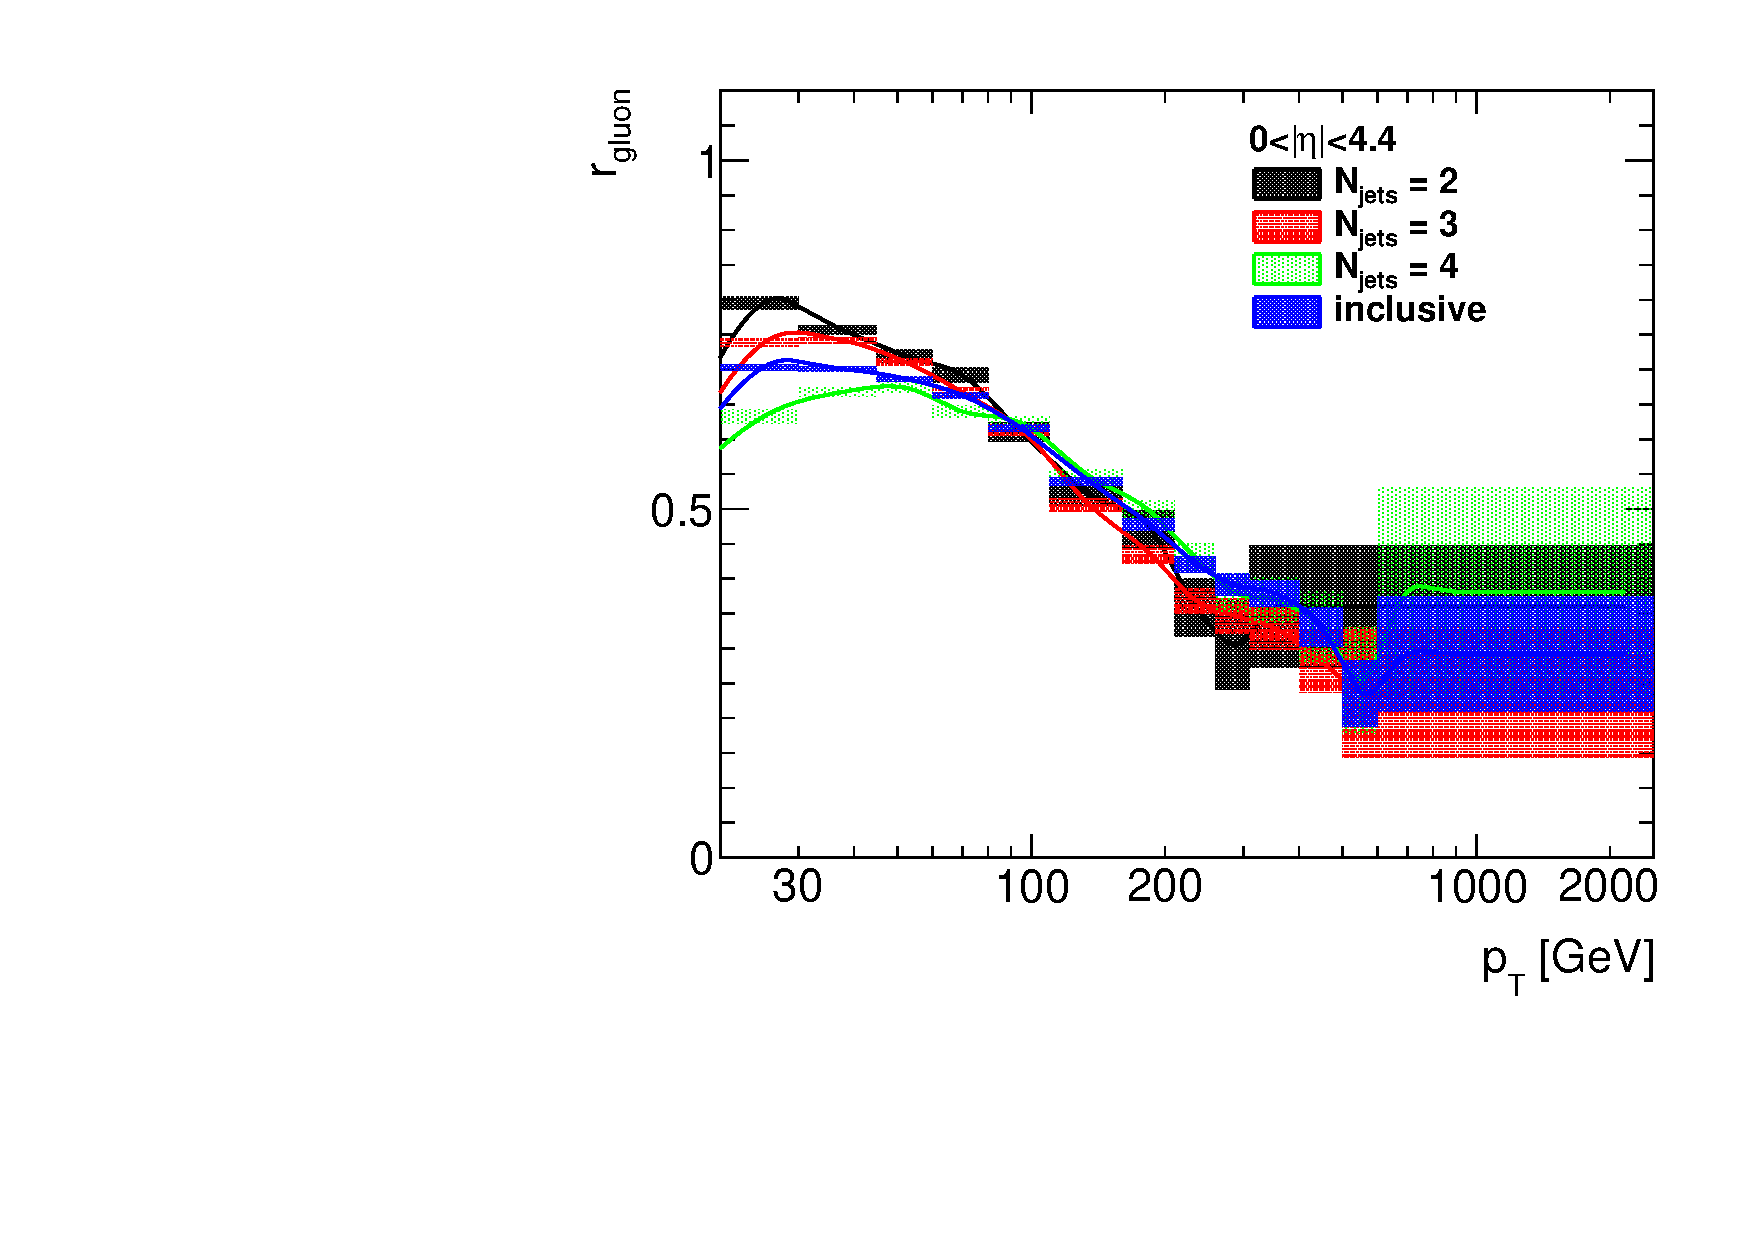
\includegraphics[width=0.49\textwidth]{figs/fractions_1d_dilep.pdf}
	\label{sfig:qgf7TeV1d}
}
\subfloat[\gls{QGF} as a function of the jet \pt\ and $\eta$]{
	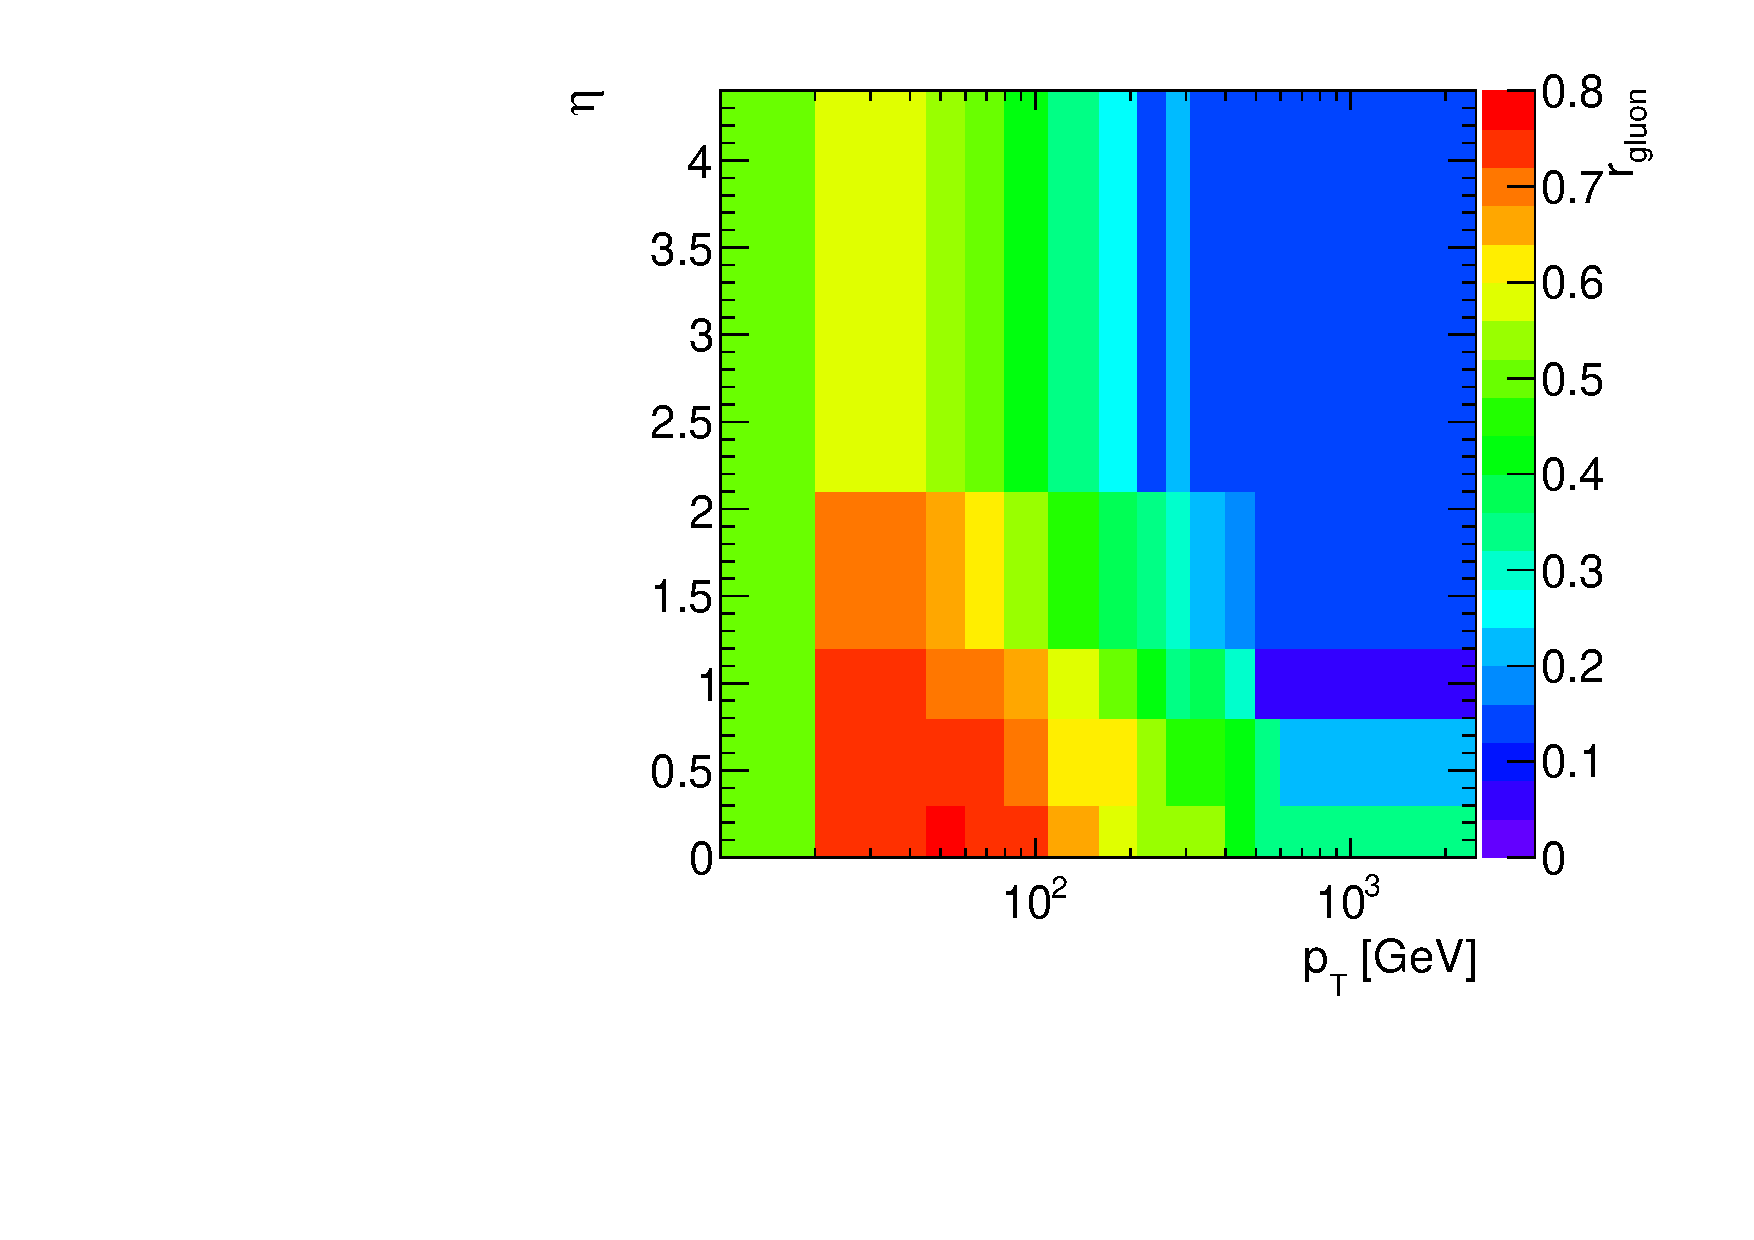
\includegraphics[width=0.49\textwidth]{figs/qgf_2d_dilep.pdf}
	% \includegraphics[width=0.49\textwidth]{figs/qgf_2d_dilep_njet2.pdf}
	\label{sfig:qgf7TeV2d}
}
\caption[\gls{QGF} for $\sqrts=7$~\TeV\ data]{
The analysis-specific \gls{QGF} $r_\mathrm{gluon}$ is shown in \fig~\subref{sfig:qgf7TeV1d} in bins of jet \pt\ for different jets multiplicities. 
%
\Fig~\subref{sfig:qgf7TeV2d} shows the \gls{QGF} as a function of jet $\eta$ and \pt\ for events passing the analysis-specific jet selection requirements inclusively in jet multiplicity. 
%
\label{fig:qgf7TeV}}
\end{figure*}
%%%%%%%%%%%%%%%%%%%%%%%%%%%%%%%%%%%%%%%%%%%%%%%%%%%%%%%%%%%%%%%%%%%%%%%%%%%%%


Jets at \recolevel, passing the analysis-specific quality requirements, are matched to jets at \stablevel, referred to as truth jets, within a cone of $\dR<0.3$. 
%
Each \recolevel\ jet is assigned the flavour of the most energetic \genlevel\ particle from \gls{MC} information within a spatial distance of $\dR=0.4$ to the matched truth jet. 
%
A jet \pt, $\eta$ and jet multiplicity $\Njet{}$ dependent \gls{QGF} is determined by the ratio $r_\mathrm{gluon}=\Njet{gluon}/(\Njet{gluon}+\Njet{quark})$, with $\Njet{quark}$ being defined as the number of jets that were assigned a light quark flavour ($u$, $d$, $s$).
%
The uncertainty on the binned \gls{QGF} consists of a statistical component, determined from the number of jets observed, and a systematic component, taken from the comparison of the \gls{MC} samples used for the determination of the signal \gls{MC}, the hadronisation and the \gls{ISRFSR} uncertainties. The uncertainties are summed in quadrature to obtain the total uncertainty on the \gls{QGF} in each \pt, $\eta$ and $\Njet{}$ bin. 
%
\Fig~\subref*{sfig:qgf7TeV1d} shows the \gls{QGF} as a function of \pt. In this figure, the \gls{QGF} is integrated over jet $\eta$ and shown for different jet multiplicities. The uncertainty bands are dominated systematically in the low \pt\ regions and statistically in the high-\pt\ tails. 
%
\Fig~\subref{sfig:qgf7TeV2d} shows the \gls{QGF} as functions of jet $\eta$ and \pt\ for events passing the analysis-specific jet selection requirements inclusively in jet multiplicity. This histogram contains the necessary information for the determination of the jet flavour related uncertainties. 
%







\section{Summary}
%
The \tquark\ mass has been measured at $\sqrts=7$~\TeV\ in the \ttbarll\ channel to be $\mt = \XZ{173.79}{0.54}{1.30}~\GeV=\XZtot{173.79}{1.41}~\GeV$.  
%
The precision is limited by the systematic uncertainties related to the \gls{JES} and \gls{bJES}, while the next largest components are of statistical and theoretical nature. 
%
The statistical power of the $\sqrts=7$~\TeV\ dataset is insufficient for a further phase space optimisation to reduce the systematic components. 
%
However, this is feasible for the analysis of the $\sqrts=8$~\TeV\ \gls{ATLAS} data described next.
